\documentclass{report}

%%%%%%%%%%%%%%%%%%%%%%%%%%%%%%%%%
% PACKAGE IMPORTS
%%%%%%%%%%%%%%%%%%%%%%%%%%%%%%%%%


\usepackage[tmargin=2cm,rmargin=1in,lmargin=1in,margin=0.85in,bmargin=2cm,footskip=.2in]{geometry}
\usepackage{amsmath,amsfonts,amsthm,amssymb,mathtools}
\usepackage[varbb]{newpxmath}
\usepackage{xfrac}
\usepackage{float}
\usepackage[makeroom]{cancel}
\usepackage{mathtools}
\usepackage{bookmark}
\usepackage{enumitem}
\usepackage{hyperref,theoremref}
\hypersetup{
	pdftitle={Assignment},
	colorlinks=true, linkcolor=doc!90,
	bookmarksnumbered=true,
	bookmarksopen=true
}
\usepackage[most,many,breakable]{tcolorbox}
\usepackage{xcolor}
\usepackage{varwidth}
\usepackage{varwidth}
\usepackage{etoolbox}
%\usepackage{authblk}
\usepackage{nameref}
\usepackage{multicol,array}
\usepackage{tikz-cd}
\usepackage[ruled,vlined,linesnumbered]{algorithm2e}
\usepackage{comment} % enables the use of multi-line comments (\ifx \fi) 
\usepackage{import}
\usepackage{xifthen}
\usepackage{pdfpages}
\usepackage{transparent}

\newcommand\mycommfont[1]{\footnotesize\ttfamily\textcolor{blue}{#1}}
\SetCommentSty{mycommfont}
\newcommand{\incfig}[1]{%
    \def\svgwidth{\columnwidth}
    \import{./figures/}{#1.pdf_tex}
}

\usepackage{tikzsymbols}
\renewcommand\qedsymbol{$\Laughey$}


%\usepackage{import}
%\usepackage{xifthen}
%\usepackage{pdfpages}
%\usepackage{transparent}


%%%%%%%%%%%%%%%%%%%%%%%%%%%%%%
% SELF MADE COLORS
%%%%%%%%%%%%%%%%%%%%%%%%%%%%%%



\definecolor{myg}{RGB}{56, 140, 70}
\definecolor{myb}{RGB}{45, 111, 177}
\definecolor{myr}{RGB}{199, 68, 64}
\definecolor{mytheorembg}{HTML}{F2F2F9}
\definecolor{mytheoremfr}{HTML}{00007B}
\definecolor{mylenmabg}{HTML}{FFFAF8}
\definecolor{mylenmafr}{HTML}{983b0f}
\definecolor{mypropbg}{HTML}{f2fbfc}
\definecolor{mypropfr}{HTML}{191971}
\definecolor{myexamplebg}{HTML}{F2FBF8}
\definecolor{myexamplefr}{HTML}{88D6D1}
\definecolor{myexampleti}{HTML}{2A7F7F}
\definecolor{mydefinitbg}{HTML}{E5E5FF}
\definecolor{mydefinitfr}{HTML}{3F3FA3}
\definecolor{notesgreen}{RGB}{0,162,0}
\definecolor{myp}{RGB}{197, 92, 212}
\definecolor{mygr}{HTML}{2C3338}
\definecolor{myred}{RGB}{127,0,0}
\definecolor{myyellow}{RGB}{169,121,69}
\definecolor{myexercisebg}{HTML}{F2FBF8}
\definecolor{myexercisefg}{HTML}{88D6D1}


%%%%%%%%%%%%%%%%%%%%%%%%%%%%
% TCOLORBOX SETUPS
%%%%%%%%%%%%%%%%%%%%%%%%%%%%

\setlength{\parindent}{1cm}
%================================
% THEOREM BOX
%================================

\tcbuselibrary{theorems,skins,hooks}
\newtcbtheorem[number within=section]{Theorem}{Theorem}
{%
	enhanced,
	breakable,
	colback = mytheorembg,
	frame hidden,
	boxrule = 0sp,
	borderline west = {2pt}{0pt}{mytheoremfr},
	sharp corners,
	detach title,
	before upper = \tcbtitle\par\smallskip,
	coltitle = mytheoremfr,
	fonttitle = \bfseries\sffamily,
	description font = \mdseries,
	separator sign none,
	segmentation style={solid, mytheoremfr},
}
{th}

\tcbuselibrary{theorems,skins,hooks}
\newtcbtheorem[number within=chapter]{theorem}{Theorem}
{%
	enhanced,
	breakable,
	colback = mytheorembg,
	frame hidden,
	boxrule = 0sp,
	borderline west = {2pt}{0pt}{mytheoremfr},
	sharp corners,
	detach title,
	before upper = \tcbtitle\par\smallskip,
	coltitle = mytheoremfr,
	fonttitle = \bfseries\sffamily,
	description font = \mdseries,
	separator sign none,
	segmentation style={solid, mytheoremfr},
}
{th}


\tcbuselibrary{theorems,skins,hooks}
\newtcolorbox{Theoremcon}
{%
	enhanced
	,breakable
	,colback = mytheorembg
	,frame hidden
	,boxrule = 0sp
	,borderline west = {2pt}{0pt}{mytheoremfr}
	,sharp corners
	,description font = \mdseries
	,separator sign none
}

%================================
% Corollery
%================================
\tcbuselibrary{theorems,skins,hooks}
\newtcbtheorem[number within=section]{Corollary}{Corollary}
{%
	enhanced
	,breakable
	,colback = myp!10
	,frame hidden
	,boxrule = 0sp
	,borderline west = {2pt}{0pt}{myp!85!black}
	,sharp corners
	,detach title
	,before upper = \tcbtitle\par\smallskip
	,coltitle = myp!85!black
	,fonttitle = \bfseries\sffamily
	,description font = \mdseries
	,separator sign none
	,segmentation style={solid, myp!85!black}
}
{th}
\tcbuselibrary{theorems,skins,hooks}
\newtcbtheorem[number within=chapter]{corollary}{Corollary}
{%
	enhanced
	,breakable
	,colback = myp!10
	,frame hidden
	,boxrule = 0sp
	,borderline west = {2pt}{0pt}{myp!85!black}
	,sharp corners
	,detach title
	,before upper = \tcbtitle\par\smallskip
	,coltitle = myp!85!black
	,fonttitle = \bfseries\sffamily
	,description font = \mdseries
	,separator sign none
	,segmentation style={solid, myp!85!black}
}
{th}


%================================
% LENMA
%================================

\tcbuselibrary{theorems,skins,hooks}
\newtcbtheorem[number within=section]{Lenma}{Lenma}
{%
	enhanced,
	breakable,
	colback = mylenmabg,
	frame hidden,
	boxrule = 0sp,
	borderline west = {2pt}{0pt}{mylenmafr},
	sharp corners,
	detach title,
	before upper = \tcbtitle\par\smallskip,
	coltitle = mylenmafr,
	fonttitle = \bfseries\sffamily,
	description font = \mdseries,
	separator sign none,
	segmentation style={solid, mylenmafr},
}
{th}

\tcbuselibrary{theorems,skins,hooks}
\newtcbtheorem[number within=chapter]{lenma}{Lenma}
{%
	enhanced,
	breakable,
	colback = mylenmabg,
	frame hidden,
	boxrule = 0sp,
	borderline west = {2pt}{0pt}{mylenmafr},
	sharp corners,
	detach title,
	before upper = \tcbtitle\par\smallskip,
	coltitle = mylenmafr,
	fonttitle = \bfseries\sffamily,
	description font = \mdseries,
	separator sign none,
	segmentation style={solid, mylenmafr},
}
{th}


%================================
% PROPOSITION
%================================

\tcbuselibrary{theorems,skins,hooks}
\newtcbtheorem[number within=section]{Prop}{Proposition}
{%
	enhanced,
	breakable,
	colback = mypropbg,
	frame hidden,
	boxrule = 0sp,
	borderline west = {2pt}{0pt}{mypropfr},
	sharp corners,
	detach title,
	before upper = \tcbtitle\par\smallskip,
	coltitle = mypropfr,
	fonttitle = \bfseries\sffamily,
	description font = \mdseries,
	separator sign none,
	segmentation style={solid, mypropfr},
}
{th}

\tcbuselibrary{theorems,skins,hooks}
\newtcbtheorem[number within=chapter]{prop}{Proposition}
{%
	enhanced,
	breakable,
	colback = mypropbg,
	frame hidden,
	boxrule = 0sp,
	borderline west = {2pt}{0pt}{mypropfr},
	sharp corners,
	detach title,
	before upper = \tcbtitle\par\smallskip,
	coltitle = mypropfr,
	fonttitle = \bfseries\sffamily,
	description font = \mdseries,
	separator sign none,
	segmentation style={solid, mypropfr},
}
{th}


%================================
% CLAIM
%================================

\tcbuselibrary{theorems,skins,hooks}
\newtcbtheorem[number within=section]{claim}{Claim}
{%
	enhanced
	,breakable
	,colback = myg!10
	,frame hidden
	,boxrule = 0sp
	,borderline west = {2pt}{0pt}{myg}
	,sharp corners
	,detach title
	,before upper = \tcbtitle\par\smallskip
	,coltitle = myg!85!black
	,fonttitle = \bfseries\sffamily
	,description font = \mdseries
	,separator sign none
	,segmentation style={solid, myg!85!black}
}
{th}



%================================
% Exercise
%================================

\tcbuselibrary{theorems,skins,hooks}
\newtcbtheorem[number within=section]{Exercise}{Exercise}
{%
	enhanced,
	breakable,
	colback = myexercisebg,
	frame hidden,
	boxrule = 0sp,
	borderline west = {2pt}{0pt}{myexercisefg},
	sharp corners,
	detach title,
	before upper = \tcbtitle\par\smallskip,
	coltitle = myexercisefg,
	fonttitle = \bfseries\sffamily,
	description font = \mdseries,
	separator sign none,
	segmentation style={solid, myexercisefg},
}
{th}

\tcbuselibrary{theorems,skins,hooks}
\newtcbtheorem[number within=chapter]{exercise}{Exercise}
{%
	enhanced,
	breakable,
	colback = myexercisebg,
	frame hidden,
	boxrule = 0sp,
	borderline west = {2pt}{0pt}{myexercisefg},
	sharp corners,
	detach title,
	before upper = \tcbtitle\par\smallskip,
	coltitle = myexercisefg,
	fonttitle = \bfseries\sffamily,
	description font = \mdseries,
	separator sign none,
	segmentation style={solid, myexercisefg},
}
{th}

%================================
% EXAMPLE BOX
%================================

\newtcbtheorem[number within=section]{Example}{Example}
{%
	colback = myexamplebg
	,breakable
	,colframe = myexamplefr
	,coltitle = myexampleti
	,boxrule = 1pt
	,sharp corners
	,detach title
	,before upper=\tcbtitle\par\smallskip
	,fonttitle = \bfseries
	,description font = \mdseries
	,separator sign none
	,description delimiters parenthesis
}
{ex}

\newtcbtheorem[number within=chapter]{example}{Example}
{%
	colback = myexamplebg
	,breakable
	,colframe = myexamplefr
	,coltitle = myexampleti
	,boxrule = 1pt
	,sharp corners
	,detach title
	,before upper=\tcbtitle\par\smallskip
	,fonttitle = \bfseries
	,description font = \mdseries
	,separator sign none
	,description delimiters parenthesis
}
{ex}

%================================
% DEFINITION BOX
%================================

\newtcbtheorem[number within=section]{Definition}{Definition}{enhanced,
	before skip=2mm,after skip=2mm, colback=red!5,colframe=red!80!black,boxrule=0.5mm,
	attach boxed title to top left={xshift=1cm,yshift*=1mm-\tcboxedtitleheight}, varwidth boxed title*=-3cm,
	boxed title style={frame code={
					\path[fill=tcbcolback]
					([yshift=-1mm,xshift=-1mm]frame.north west)
					arc[start angle=0,end angle=180,radius=1mm]
					([yshift=-1mm,xshift=1mm]frame.north east)
					arc[start angle=180,end angle=0,radius=1mm];
					\path[left color=tcbcolback!60!black,right color=tcbcolback!60!black,
						middle color=tcbcolback!80!black]
					([xshift=-2mm]frame.north west) -- ([xshift=2mm]frame.north east)
					[rounded corners=1mm]-- ([xshift=1mm,yshift=-1mm]frame.north east)
					-- (frame.south east) -- (frame.south west)
					-- ([xshift=-1mm,yshift=-1mm]frame.north west)
					[sharp corners]-- cycle;
				},interior engine=empty,
		},
	fonttitle=\bfseries,
	title={#2},#1}{def}
\newtcbtheorem[number within=chapter]{definition}{Definition}{enhanced,
	before skip=2mm,after skip=2mm, colback=red!5,colframe=red!80!black,boxrule=0.5mm,
	attach boxed title to top left={xshift=1cm,yshift*=1mm-\tcboxedtitleheight}, varwidth boxed title*=-3cm,
	boxed title style={frame code={
					\path[fill=tcbcolback]
					([yshift=-1mm,xshift=-1mm]frame.north west)
					arc[start angle=0,end angle=180,radius=1mm]
					([yshift=-1mm,xshift=1mm]frame.north east)
					arc[start angle=180,end angle=0,radius=1mm];
					\path[left color=tcbcolback!60!black,right color=tcbcolback!60!black,
						middle color=tcbcolback!80!black]
					([xshift=-2mm]frame.north west) -- ([xshift=2mm]frame.north east)
					[rounded corners=1mm]-- ([xshift=1mm,yshift=-1mm]frame.north east)
					-- (frame.south east) -- (frame.south west)
					-- ([xshift=-1mm,yshift=-1mm]frame.north west)
					[sharp corners]-- cycle;
				},interior engine=empty,
		},
	fonttitle=\bfseries,
	title={#2},#1}{def}



%================================
% Solution BOX
%================================

\makeatletter
\newtcbtheorem{question}{Question}{enhanced,
	breakable,
	colback=white,
	colframe=myb!80!black,
	attach boxed title to top left={yshift*=-\tcboxedtitleheight},
	fonttitle=\bfseries,
	title={#2},
	boxed title size=title,
	boxed title style={%
			sharp corners,
			rounded corners=northwest,
			colback=tcbcolframe,
			boxrule=0pt,
		},
	underlay boxed title={%
			\path[fill=tcbcolframe] (title.south west)--(title.south east)
			to[out=0, in=180] ([xshift=5mm]title.east)--
			(title.center-|frame.east)
			[rounded corners=\kvtcb@arc] |-
			(frame.north) -| cycle;
		},
	#1
}{def}
\makeatother

%================================
% SOLUTION BOX
%================================

\makeatletter
\newtcolorbox{solution}{enhanced,
	breakable,
	colback=white,
	colframe=myg!80!black,
	attach boxed title to top left={yshift*=-\tcboxedtitleheight},
	title=Solution,
	boxed title size=title,
	boxed title style={%
			sharp corners,
			rounded corners=northwest,
			colback=tcbcolframe,
			boxrule=0pt,
		},
	underlay boxed title={%
			\path[fill=tcbcolframe] (title.south west)--(title.south east)
			to[out=0, in=180] ([xshift=5mm]title.east)--
			(title.center-|frame.east)
			[rounded corners=\kvtcb@arc] |-
			(frame.north) -| cycle;
		},
}
\makeatother

%================================
% Question BOX
%================================

\makeatletter
\newtcbtheorem{qstion}{Question}{enhanced,
	breakable,
	colback=white,
	colframe=mygr,
	attach boxed title to top left={yshift*=-\tcboxedtitleheight},
	fonttitle=\bfseries,
	title={#2},
	boxed title size=title,
	boxed title style={%
			sharp corners,
			rounded corners=northwest,
			colback=tcbcolframe,
			boxrule=0pt,
		},
	underlay boxed title={%
			\path[fill=tcbcolframe] (title.south west)--(title.south east)
			to[out=0, in=180] ([xshift=5mm]title.east)--
			(title.center-|frame.east)
			[rounded corners=\kvtcb@arc] |-
			(frame.north) -| cycle;
		},
	#1
}{def}
\makeatother

\newtcbtheorem[number within=chapter]{wconc}{Wrong Concept}{
	breakable,
	enhanced,
	colback=white,
	colframe=myr,
	arc=0pt,
	outer arc=0pt,
	fonttitle=\bfseries\sffamily\large,
	colbacktitle=myr,
	attach boxed title to top left={},
	boxed title style={
			enhanced,
			skin=enhancedfirst jigsaw,
			arc=3pt,
			bottom=0pt,
			interior style={fill=myr}
		},
	#1
}{def}



%================================
% NOTE BOX
%================================

\usetikzlibrary{arrows,calc,shadows.blur}
\tcbuselibrary{skins}
\newtcolorbox{note}[1][]{%
	enhanced jigsaw,
	colback=gray!20!white,%
	colframe=gray!80!black,
	size=small,
	boxrule=1pt,
	title=\textbf{Note:-},
	halign title=flush center,
	coltitle=black,
	breakable,
	drop shadow=black!50!white,
	attach boxed title to top left={xshift=1cm,yshift=-\tcboxedtitleheight/2,yshifttext=-\tcboxedtitleheight/2},
	minipage boxed title=1.5cm,
	boxed title style={%
			colback=white,
			size=fbox,
			boxrule=1pt,
			boxsep=2pt,
			underlay={%
					\coordinate (dotA) at ($(interior.west) + (-0.5pt,0)$);
					\coordinate (dotB) at ($(interior.east) + (0.5pt,0)$);
					\begin{scope}
						\clip (interior.north west) rectangle ([xshift=3ex]interior.east);
						\filldraw [white, blur shadow={shadow opacity=60, shadow yshift=-.75ex}, rounded corners=2pt] (interior.north west) rectangle (interior.south east);
					\end{scope}
					\begin{scope}[gray!80!black]
						\fill (dotA) circle (2pt);
						\fill (dotB) circle (2pt);
					\end{scope}
				},
		},
	#1,
}

%%%%%%%%%%%%%%%%%%%%%%%%%%%%%%
% SELF MADE COMMANDS
%%%%%%%%%%%%%%%%%%%%%%%%%%%%%%


\newcommand{\thm}[2]{\begin{Theorem}{#1}{}#2\end{Theorem}}
\newcommand{\cor}[2]{\begin{Corollary}{#1}{}#2\end{Corollary}}
\newcommand{\mlenma}[2]{\begin{Lenma}{#1}{}#2\end{Lenma}}
\newcommand{\mprop}[2]{\begin{Prop}{#1}{}#2\end{Prop}}
\newcommand{\clm}[3]{\begin{claim}{#1}{#2}#3\end{claim}}
\newcommand{\wc}[2]{\begin{wconc}{#1}{}\setlength{\parindent}{1cm}#2\end{wconc}}
\newcommand{\thmcon}[1]{\begin{Theoremcon}{#1}\end{Theoremcon}}
\newcommand{\ex}[2]{\begin{Example}{#1}{}#2\end{Example}}
\newcommand{\dfn}[2]{\begin{Definition}[colbacktitle=red!75!black]{#1}{}#2\end{Definition}}
\newcommand{\dfnc}[2]{\begin{definition}[colbacktitle=red!75!black]{#1}{}#2\end{definition}}
\newcommand{\qs}[2]{\begin{question}{#1}{}#2\end{question}}
\newcommand{\pf}[2]{\begin{myproof}[#1]#2\end{myproof}}
\newcommand{\nt}[1]{\begin{note}#1\end{note}}

\newcommand*\circled[1]{\tikz[baseline=(char.base)]{
		\node[shape=circle,draw,inner sep=1pt] (char) {#1};}}
\newcommand\getcurrentref[1]{%
	\ifnumequal{\value{#1}}{0}
	{??}
	{\the\value{#1}}%
}
\newcommand{\getCurrentSectionNumber}{\getcurrentref{section}}
\newenvironment{myproof}[1][\proofname]{%
  \proof[\bfseries #1: ]\color{gray}%
}{\endproof}

\newcommand{\mclm}[2]{\begin{myclaim}[#1]#2\end{myclaim}}
\newenvironment{myclaim}[1][\claimname]{\proof[\bfseries #1: ]}{}

\newcounter{mylabelcounter}

\makeatletter
\newcommand{\setword}[2]{%
	\phantomsection
	#1\def\@currentlabel{\unexpanded{#1}}\label{#2}%
}
\makeatother




\tikzset{
	symbol/.style={
			draw=none,
			every to/.append style={
					edge node={node [sloped, allow upside down, auto=false]{$#1$}}}
		}
}


% deliminators
\DeclarePairedDelimiter{\abs}{\lvert}{\rvert}
\DeclarePairedDelimiter{\norm}{\lVert}{\rVert}

\DeclarePairedDelimiter{\ceil}{\lceil}{\rceil}
\DeclarePairedDelimiter{\floor}{\lfloor}{\rfloor}
\DeclarePairedDelimiter{\round}{\lfloor}{\rceil}

\newsavebox\diffdbox
\newcommand{\slantedromand}{{\mathpalette\makesl{d}}}
\newcommand{\makesl}[2]{%
\begingroup
\sbox{\diffdbox}{$\mathsurround=0pt#1\mathrm{#2}$}%
\pdfsave
\pdfsetmatrix{1 0 0.2 1}%
\rlap{\usebox{\diffdbox}}%
\pdfrestore
\hskip\wd\diffdbox
\endgroup
}
\newcommand{\dd}[1][]{\ensuremath{\mathop{}\!\ifstrempty{#1}{%
\slantedromand\@ifnextchar^{\hspace{0.2ex}}{\hspace{0.1ex}}}%
{\slantedromand\hspace{0.2ex}^{#1}}}}
\ProvideDocumentCommand\dv{o m g}{%
  \ensuremath{%
    \IfValueTF{#3}{%
      \IfNoValueTF{#1}{%
        \frac{\dd #2}{\dd #3}%
      }{%
        \frac{\dd^{#1} #2}{\dd #3^{#1}}%
      }%
    }{%
      \IfNoValueTF{#1}{%
        \frac{\dd}{\dd #2}%
      }{%
        \frac{\dd^{#1}}{\dd #2^{#1}}%
      }%
    }%
  }%
}
\providecommand*{\pdv}[3][]{\frac{\partial^{#1}#2}{\partial#3^{#1}}}
%  - others
\DeclareMathOperator{\Lap}{\mathcal{L}}
\DeclareMathOperator{\Var}{Var} % varience
\DeclareMathOperator{\Cov}{Cov} % covarience
\DeclareMathOperator{\E}{E} % expected

% Since the amsthm package isn't loaded

% I prefer the slanted \leq
\let\oldleq\leq % save them in case they're every wanted
\let\oldgeq\geq
\renewcommand{\leq}{\leqslant}
\renewcommand{\geq}{\geqslant}

% % redefine matrix env to allow for alignment, use r as default
% \renewcommand*\env@matrix[1][r]{\hskip -\arraycolsep
%     \let\@ifnextchar\new@ifnextchar
%     \array{*\c@MaxMatrixCols #1}}


%\usepackage{framed}
%\usepackage{titletoc}
%\usepackage{etoolbox}
%\usepackage{lmodern}


%\patchcmd{\tableofcontents}{\contentsname}{\sffamily\contentsname}{}{}

%\renewenvironment{leftbar}
%{\def\FrameCommand{\hspace{6em}%
%		{\color{myyellow}\vrule width 2pt depth 6pt}\hspace{1em}}%
%	\MakeFramed{\parshape 1 0cm \dimexpr\textwidth-6em\relax\FrameRestore}\vskip2pt%
%}
%{\endMakeFramed}

%\titlecontents{chapter}
%[0em]{\vspace*{2\baselineskip}}
%{\parbox{4.5em}{%
%		\hfill\Huge\sffamily\bfseries\color{myred}\thecontentspage}%
%	\vspace*{-2.3\baselineskip}\leftbar\textsc{\small\chaptername~\thecontentslabel}\\\sffamily}
%{}{\endleftbar}
%\titlecontents{section}
%[8.4em]
%{\sffamily\contentslabel{3em}}{}{}
%{\hspace{0.5em}\nobreak\itshape\color{myred}\contentspage}
%\titlecontents{subsection}
%[8.4em]
%{\sffamily\contentslabel{3em}}{}{}  
%{\hspace{0.5em}\nobreak\itshape\color{myred}\contentspage}



%%%%%%%%%%%%%%%%%%%%%%%%%%%%%%%%%%%%%%%%%%%
% TABLE OF CONTENTS
%%%%%%%%%%%%%%%%%%%%%%%%%%%%%%%%%%%%%%%%%%%

\usepackage{tikz}
\definecolor{doc}{RGB}{0,60,110}
\usepackage{titletoc}
\contentsmargin{0cm}
\titlecontents{chapter}[3.7pc]
{\addvspace{30pt}%
	\begin{tikzpicture}[remember picture, overlay]%
		\draw[fill=doc!60,draw=doc!60] (-7,-.1) rectangle (-0.9,.5);%
		\pgftext[left,x=-3.5cm,y=0.2cm]{\color{white}\Large\sc\bfseries Chapter\ \thecontentslabel};%
	\end{tikzpicture}\color{doc!60}\large\sc\bfseries}%
{}
{}
{\;\titlerule\;\large\sc\bfseries Page \thecontentspage
	\begin{tikzpicture}[remember picture, overlay]
		\draw[fill=doc!60,draw=doc!60] (2pt,0) rectangle (4,0.1pt);
	\end{tikzpicture}}%
\titlecontents{section}[3.7pc]
{\addvspace{2pt}}
{\contentslabel[\thecontentslabel]{2pc}}
{}
{\hfill\small \thecontentspage}
[]
\titlecontents*{subsection}[3.7pc]
{\addvspace{-1pt}\small}
{}
{}
{\ --- \small\thecontentspage}
[ \textbullet\ ][]

\makeatletter
\renewcommand{\tableofcontents}{%
	\chapter*{%
	  \vspace*{-20\p@}%
	  \begin{tikzpicture}[remember picture, overlay]%
		  \pgftext[right,x=15cm,y=0.2cm]{\color{doc!60}\Huge\sc\bfseries \contentsname};%
		  \draw[fill=doc!60,draw=doc!60] (13,-.75) rectangle (20,1);%
		  \clip (13,-.75) rectangle (20,1);
		  \pgftext[right,x=15cm,y=0.2cm]{\color{white}\Huge\sc\bfseries \contentsname};%
	  \end{tikzpicture}}%
	\@starttoc{toc}}
\makeatother

%tikz
\tikzset{
box/.style ={
rectangle, %矩形节点
rounded corners =5pt, %圆角
minimum width =50pt, %最小宽度
minimum height =20pt, %最小高度
inner sep=5pt, %文字和边框的距离
draw=blue %边框颜色}
}
}
\definecolor{dkgreen}{rgb}{0,0.6,0}
\definecolor{gray}{rgb}{0.5,0.5,0.5}
\definecolor{mauve}{rgb}{0.58,0,0.82}
\lstset{frame=tb,
  language=Python,
  aboveskip=3mm,
  belowskip=3mm,
  showstringspaces=false,
  columns=flexible,
  basicstyle={\small\ttfamily},
  numbers=none,
  numberstyle=\tiny\color{gray},
  keywordstyle=\color{blue},
  commentstyle=\color{dkgreen},
  stringstyle=\color{mauve},
  breaklines=true,
  breakatwhitespace=true,
  tabsize=3
}

%From M275 "Topology" at SJSU
\newcommand{\id}{\mathrm{id}}
\newcommand{\taking}[1]{\xrightarrow{#1}}
\newcommand{\inv}{^{-1}}

%From M170 "Introduction to Graph Theory" at SJSU
\DeclareMathOperator{\diam}{diam}
\DeclareMathOperator{\ord}{ord}
\newcommand{\defeq}{\overset{\mathrm{def}}{=}}

%From the USAMO .tex files
\newcommand{\ts}{\textsuperscript}
\newcommand{\dg}{^\circ}
\newcommand{\ii}{\item}

% % From Math 55 and Math 145 at Harvard
% \newenvironment{subproof}[1][Proof]{%
% \begin{proof}[#1] \renewcommand{\qedsymbol}{$\blacksquare$}}%
% {\end{proof}}

\newcommand{\liff}{\leftrightarrow}
\newcommand{\lthen}{\rightarrow}
\newcommand{\opname}{\operatorname}
\newcommand{\surjto}{\twoheadrightarrow}
\newcommand{\injto}{\hookrightarrow}
\newcommand{\On}{\mathrm{On}} % ordinals
\DeclareMathOperator{\img}{im} % Image
\DeclareMathOperator{\Img}{Im} % Image
\DeclareMathOperator{\coker}{coker} % Cokernel
\DeclareMathOperator{\Coker}{Coker} % Cokernel
\DeclareMathOperator{\Ker}{Ker} % Kernel
\DeclareMathOperator{\rank}{rank}
\DeclareMathOperator{\Spec}{Spec} % spectrum
\DeclareMathOperator{\Tr}{Tr} % trace
\DeclareMathOperator{\pr}{pr} % projection
\DeclareMathOperator{\ext}{ext} % extension
\DeclareMathOperator{\pred}{pred} % predecessor
\DeclareMathOperator{\dom}{dom} % domain
\DeclareMathOperator{\ran}{ran} % range
\DeclareMathOperator{\Hom}{Hom} % homomorphism
\DeclareMathOperator{\Mor}{Mor} % morphisms
\DeclareMathOperator{\End}{End} % endomorphism

\newcommand{\eps}{\epsilon}
\newcommand{\veps}{\varepsilon}
\newcommand{\ol}{\overline}
\newcommand{\ul}{\underline}
\newcommand{\wt}{\widetilde}
\newcommand{\wh}{\widehat}
\newcommand{\vocab}[1]{\textbf{\color{blue} #1}}
\providecommand{\half}{\frac{1}{2}}
\newcommand{\dang}{\measuredangle} %% Directed angle
\newcommand{\ray}[1]{\overrightarrow{#1}}
\newcommand{\seg}[1]{\overline{#1}}
\newcommand{\arc}[1]{\wideparen{#1}}
\DeclareMathOperator{\cis}{cis}
\DeclareMathOperator*{\lcm}{lcm}
\DeclareMathOperator*{\argmin}{arg min}
\DeclareMathOperator*{\argmax}{arg max}
\newcommand{\cycsum}{\sum_{\mathrm{cyc}}}
\newcommand{\symsum}{\sum_{\mathrm{sym}}}
\newcommand{\cycprod}{\prod_{\mathrm{cyc}}}
\newcommand{\symprod}{\prod_{\mathrm{sym}}}
\newcommand{\Qed}{\begin{flushright}\qed\end{flushright}}
\newcommand{\parinn}{\setlength{\parindent}{1cm}}
\newcommand{\parinf}{\setlength{\parindent}{0cm}}
% \newcommand{\norm}{\|\cdot\|}
\newcommand{\inorm}{\norm_{\infty}}
\newcommand{\opensets}{\{V_{\alpha}\}_{\alpha\in I}}
\newcommand{\oset}{V_{\alpha}}
\newcommand{\opset}[1]{V_{\alpha_{#1}}}
\newcommand{\lub}{\text{lub}}
\newcommand{\del}[2]{\frac{\partial #1}{\partial #2}}
\newcommand{\Del}[3]{\frac{\partial^{#1} #2}{\partial^{#1} #3}}
\newcommand{\deld}[2]{\dfrac{\partial #1}{\partial #2}}
\newcommand{\Deld}[3]{\dfrac{\partial^{#1} #2}{\partial^{#1} #3}}
\newcommand{\lm}{\lambda}
\newcommand{\uin}{\mathbin{\rotatebox[origin=c]{90}{$\in$}}}
\newcommand{\usubset}{\mathbin{\rotatebox[origin=c]{90}{$\subset$}}}
\newcommand{\lt}{\left}
\newcommand{\rt}{\right}
\newcommand{\bs}[1]{\boldsymbol{#1}}
\newcommand{\exs}{\exists}
\newcommand{\st}{\strut}
\newcommand{\dps}[1]{\displaystyle{#1}}

\newcommand{\sol}{\setlength{\parindent}{0cm}\textbf{\textit{Solution:}}\setlength{\parindent}{1cm} }
\newcommand{\solve}[1]{\setlength{\parindent}{0cm}\textbf{\textit{Solution: }}\setlength{\parindent}{1cm}#1 \Qed}

% Things Lie
\newcommand{\kb}{\mathfrak b}
\newcommand{\kg}{\mathfrak g}
\newcommand{\kh}{\mathfrak h}
\newcommand{\kn}{\mathfrak n}
\newcommand{\ku}{\mathfrak u}
\newcommand{\kz}{\mathfrak z}
\DeclareMathOperator{\Ext}{Ext} % Ext functor
\DeclareMathOperator{\Tor}{Tor} % Tor functor
\newcommand{\gl}{\opname{\mathfrak{gl}}} % frak gl group
\renewcommand{\sl}{\opname{\mathfrak{sl}}} % frak sl group chktex 6

% More script letters etc.
\newcommand{\SA}{\mathcal A}
\newcommand{\SB}{\mathcal B}
\newcommand{\SC}{\mathcal C}
\newcommand{\SF}{\mathcal F}
\newcommand{\SG}{\mathcal G}
\newcommand{\SH}{\mathcal H}
\newcommand{\OO}{\mathcal O}

\newcommand{\SCA}{\mathscr A}
\newcommand{\SCB}{\mathscr B}
\newcommand{\SCC}{\mathscr C}
\newcommand{\SCD}{\mathscr D}
\newcommand{\SCE}{\mathscr E}
\newcommand{\SCF}{\mathscr F}
\newcommand{\SCG}{\mathscr G}
\newcommand{\SCH}{\mathscr H}

% Mathfrak primes
\newcommand{\km}{\mathfrak m}
\newcommand{\kp}{\mathfrak p}
\newcommand{\kq}{\mathfrak q}

% number sets
\newcommand{\RR}[1][]{\ensuremath{\ifstrempty{#1}{\mathbb{R}}{\mathbb{R}^{#1}}}}
\newcommand{\NN}[1][]{\ensuremath{\ifstrempty{#1}{\mathbb{N}}{\mathbb{N}^{#1}}}}
\newcommand{\ZZ}[1][]{\ensuremath{\ifstrempty{#1}{\mathbb{Z}}{\mathbb{Z}^{#1}}}}
\newcommand{\QQ}[1][]{\ensuremath{\ifstrempty{#1}{\mathbb{Q}}{\mathbb{Q}^{#1}}}}
\newcommand{\CC}[1][]{\ensuremath{\ifstrempty{#1}{\mathbb{C}}{\mathbb{C}^{#1}}}}
\newcommand{\PP}[1][]{\ensuremath{\ifstrempty{#1}{\mathbb{P}}{\mathbb{P}^{#1}}}}
\newcommand{\HH}[1][]{\ensuremath{\ifstrempty{#1}{\mathbb{H}}{\mathbb{H}^{#1}}}}
\newcommand{\FF}[1][]{\ensuremath{\ifstrempty{#1}{\mathbb{F}}{\mathbb{F}^{#1}}}}
% expected value
\newcommand{\EE}{\ensuremath{\mathbb{E}}}
\newcommand{\charin}{\text{ char }}
\DeclareMathOperator{\sign}{sign}
\DeclareMathOperator{\Aut}{Aut}
\DeclareMathOperator{\Inn}{Inn}
\DeclareMathOperator{\Syl}{Syl}
\DeclareMathOperator{\Gal}{Gal}
\DeclareMathOperator{\GL}{GL} % General linear group
\DeclareMathOperator{\SL}{SL} % Special linear group

%---------------------------------------
% BlackBoard Math Fonts :-
%---------------------------------------

%Captital Letters
\newcommand{\bbA}{\mathbb{A}}	\newcommand{\bbB}{\mathbb{B}}
\newcommand{\bbC}{\mathbb{C}}	\newcommand{\bbD}{\mathbb{D}}
\newcommand{\bbE}{\mathbb{E}}	\newcommand{\bbF}{\mathbb{F}}
\newcommand{\bbG}{\mathbb{G}}	\newcommand{\bbH}{\mathbb{H}}
\newcommand{\bbI}{\mathbb{I}}	\newcommand{\bbJ}{\mathbb{J}}
\newcommand{\bbK}{\mathbb{K}}	\newcommand{\bbL}{\mathbb{L}}
\newcommand{\bbM}{\mathbb{M}}	\newcommand{\bbN}{\mathbb{N}}
\newcommand{\bbO}{\mathbb{O}}	\newcommand{\bbP}{\mathbb{P}}
\newcommand{\bbQ}{\mathbb{Q}}	\newcommand{\bbR}{\mathbb{R}}
\newcommand{\bbS}{\mathbb{S}}	\newcommand{\bbT}{\mathbb{T}}
\newcommand{\bbU}{\mathbb{U}}	\newcommand{\bbV}{\mathbb{V}}
\newcommand{\bbW}{\mathbb{W}}	\newcommand{\bbX}{\mathbb{X}}
\newcommand{\bbY}{\mathbb{Y}}	\newcommand{\bbZ}{\mathbb{Z}}

%---------------------------------------
% MathCal Fonts :-
%---------------------------------------

%Captital Letters
\newcommand{\mcA}{\mathcal{A}}	\newcommand{\mcB}{\mathcal{B}}
\newcommand{\mcC}{\mathcal{C}}	\newcommand{\mcD}{\mathcal{D}}
\newcommand{\mcE}{\mathcal{E}}	\newcommand{\mcF}{\mathcal{F}}
\newcommand{\mcG}{\mathcal{G}}	\newcommand{\mcH}{\mathcal{H}}
\newcommand{\mcI}{\mathcal{I}}	\newcommand{\mcJ}{\mathcal{J}}
\newcommand{\mcK}{\mathcal{K}}	\newcommand{\mcL}{\mathcal{L}}
\newcommand{\mcM}{\mathcal{M}}	\newcommand{\mcN}{\mathcal{N}}
\newcommand{\mcO}{\mathcal{O}}	\newcommand{\mcP}{\mathcal{P}}
\newcommand{\mcQ}{\mathcal{Q}}	\newcommand{\mcR}{\mathcal{R}}
\newcommand{\mcS}{\mathcal{S}}	\newcommand{\mcT}{\mathcal{T}}
\newcommand{\mcU}{\mathcal{U}}	\newcommand{\mcV}{\mathcal{V}}
\newcommand{\mcW}{\mathcal{W}}	\newcommand{\mcX}{\mathcal{X}}
\newcommand{\mcY}{\mathcal{Y}}	\newcommand{\mcZ}{\mathcal{Z}}


%---------------------------------------
% Bold Math Fonts :-
%---------------------------------------

%Captital Letters
\newcommand{\bmA}{\boldsymbol{A}}	\newcommand{\bmB}{\boldsymbol{B}}
\newcommand{\bmC}{\boldsymbol{C}}	\newcommand{\bmD}{\boldsymbol{D}}
\newcommand{\bmE}{\boldsymbol{E}}	\newcommand{\bmF}{\boldsymbol{F}}
\newcommand{\bmG}{\boldsymbol{G}}	\newcommand{\bmH}{\boldsymbol{H}}
\newcommand{\bmI}{\boldsymbol{I}}	\newcommand{\bmJ}{\boldsymbol{J}}
\newcommand{\bmK}{\boldsymbol{K}}	\newcommand{\bmL}{\boldsymbol{L}}
\newcommand{\bmM}{\boldsymbol{M}}	\newcommand{\bmN}{\boldsymbol{N}}
\newcommand{\bmO}{\boldsymbol{O}}	\newcommand{\bmP}{\boldsymbol{P}}
\newcommand{\bmQ}{\boldsymbol{Q}}	\newcommand{\bmR}{\boldsymbol{R}}
\newcommand{\bmS}{\boldsymbol{S}}	\newcommand{\bmT}{\boldsymbol{T}}
\newcommand{\bmU}{\boldsymbol{U}}	\newcommand{\bmV}{\boldsymbol{V}}
\newcommand{\bmW}{\boldsymbol{W}}	\newcommand{\bmX}{\boldsymbol{X}}
\newcommand{\bmY}{\boldsymbol{Y}}	\newcommand{\bmZ}{\boldsymbol{Z}}
%Small Letters
\newcommand{\bma}{\boldsymbol{a}}	\newcommand{\bmb}{\boldsymbol{b}}
\newcommand{\bmc}{\boldsymbol{c}}	\newcommand{\bmd}{\boldsymbol{d}}
\newcommand{\bme}{\boldsymbol{e}}	\newcommand{\bmf}{\boldsymbol{f}}
\newcommand{\bmg}{\boldsymbol{g}}	\newcommand{\bmh}{\boldsymbol{h}}
\newcommand{\bmi}{\boldsymbol{i}}	\newcommand{\bmj}{\boldsymbol{j}}
\newcommand{\bmk}{\boldsymbol{k}}	\newcommand{\bml}{\boldsymbol{l}}
\newcommand{\bmm}{\boldsymbol{m}}	\newcommand{\bmn}{\boldsymbol{n}}
\newcommand{\bmo}{\boldsymbol{o}}	\newcommand{\bmp}{\boldsymbol{p}}
\newcommand{\bmq}{\boldsymbol{q}}	\newcommand{\bmr}{\boldsymbol{r}}
\newcommand{\bms}{\boldsymbol{s}}	\newcommand{\bmt}{\boldsymbol{t}}
\newcommand{\bmu}{\boldsymbol{u}}	\newcommand{\bmv}{\boldsymbol{v}}
\newcommand{\bmw}{\boldsymbol{w}}	\newcommand{\bmx}{\boldsymbol{x}}
\newcommand{\bmy}{\boldsymbol{y}}	\newcommand{\bmz}{\boldsymbol{z}}

%---------------------------------------
% Scr Math Fonts :-
%---------------------------------------

\newcommand{\sA}{{\mathscr{A}}}   \newcommand{\sB}{{\mathscr{B}}}
\newcommand{\sC}{{\mathscr{C}}}   \newcommand{\sD}{{\mathscr{D}}}
\newcommand{\sE}{{\mathscr{E}}}   \newcommand{\sF}{{\mathscr{F}}}
\newcommand{\sG}{{\mathscr{G}}}   \newcommand{\sH}{{\mathscr{H}}}
\newcommand{\sI}{{\mathscr{I}}}   \newcommand{\sJ}{{\mathscr{J}}}
\newcommand{\sK}{{\mathscr{K}}}   \newcommand{\sL}{{\mathscr{L}}}
\newcommand{\sM}{{\mathscr{M}}}   \newcommand{\sN}{{\mathscr{N}}}
\newcommand{\sO}{{\mathscr{O}}}   \newcommand{\sP}{{\mathscr{P}}}
\newcommand{\sQ}{{\mathscr{Q}}}   \newcommand{\sR}{{\mathscr{R}}}
\newcommand{\sS}{{\mathscr{S}}}   \newcommand{\sT}{{\mathscr{T}}}
\newcommand{\sU}{{\mathscr{U}}}   \newcommand{\sV}{{\mathscr{V}}}
\newcommand{\sW}{{\mathscr{W}}}   \newcommand{\sX}{{\mathscr{X}}}
\newcommand{\sY}{{\mathscr{Y}}}   \newcommand{\sZ}{{\mathscr{Z}}}


%---------------------------------------
% Math Fraktur Font
%---------------------------------------

%Captital Letters
\newcommand{\mfA}{\mathfrak{A}}	\newcommand{\mfB}{\mathfrak{B}}
\newcommand{\mfC}{\mathfrak{C}}	\newcommand{\mfD}{\mathfrak{D}}
\newcommand{\mfE}{\mathfrak{E}}	\newcommand{\mfF}{\mathfrak{F}}
\newcommand{\mfG}{\mathfrak{G}}	\newcommand{\mfH}{\mathfrak{H}}
\newcommand{\mfI}{\mathfrak{I}}	\newcommand{\mfJ}{\mathfrak{J}}
\newcommand{\mfK}{\mathfrak{K}}	\newcommand{\mfL}{\mathfrak{L}}
\newcommand{\mfM}{\mathfrak{M}}	\newcommand{\mfN}{\mathfrak{N}}
\newcommand{\mfO}{\mathfrak{O}}	\newcommand{\mfP}{\mathfrak{P}}
\newcommand{\mfQ}{\mathfrak{Q}}	\newcommand{\mfR}{\mathfrak{R}}
\newcommand{\mfS}{\mathfrak{S}}	\newcommand{\mfT}{\mathfrak{T}}
\newcommand{\mfU}{\mathfrak{U}}	\newcommand{\mfV}{\mathfrak{V}}
\newcommand{\mfW}{\mathfrak{W}}	\newcommand{\mfX}{\mathfrak{X}}
\newcommand{\mfY}{\mathfrak{Y}}	\newcommand{\mfZ}{\mathfrak{Z}}
%Small Letters
\newcommand{\mfa}{\mathfrak{a}}	\newcommand{\mfb}{\mathfrak{b}}
\newcommand{\mfc}{\mathfrak{c}}	\newcommand{\mfd}{\mathfrak{d}}
\newcommand{\mfe}{\mathfrak{e}}	\newcommand{\mff}{\mathfrak{f}}
\newcommand{\mfg}{\mathfrak{g}}	\newcommand{\mfh}{\mathfrak{h}}
\newcommand{\mfi}{\mathfrak{i}}	\newcommand{\mfj}{\mathfrak{j}}
\newcommand{\mfk}{\mathfrak{k}}	\newcommand{\mfl}{\mathfrak{l}}
\newcommand{\mfm}{\mathfrak{m}}	\newcommand{\mfn}{\mathfrak{n}}
\newcommand{\mfo}{\mathfrak{o}}	\newcommand{\mfp}{\mathfrak{p}}
\newcommand{\mfq}{\mathfrak{q}}	\newcommand{\mfr}{\mathfrak{r}}
\newcommand{\mfs}{\mathfrak{s}}	\newcommand{\mft}{\mathfrak{t}}
\newcommand{\mfu}{\mathfrak{u}}	\newcommand{\mfv}{\mathfrak{v}}
\newcommand{\mfw}{\mathfrak{w}}	\newcommand{\mfx}{\mathfrak{x}}
\newcommand{\mfy}{\mathfrak{y}}	\newcommand{\mfz}{\mathfrak{z}}


\title{\Huge{Thermodynamique}}
\author{\huge{Brandon LIN}}
\date{\today}

\begin{document}

\maketitle
\newpage% or \cleardoublepage
% \pdfbookmark[<level>]{<title>}{<dest>}
\pdfbookmark[section]{\contentsname}{toc}
\tableofcontents
\pagebreak


\chapter{Pression des fluides} % (fold)
\label{chap:Pression des fluides}

\section{Pression} % (fold)
\label{sec:Pression}

\subsection{Force de pression} % (fold)
\label{sub:Force de pression}

% subsection Force de pression (end)
\begin{equation}
  \mathrm{d} \overrightarrow{F _{\text{fluide} \to \Sigma}}= - p \mathrm{d}\overrightarrow{S} _{ext}
\end{equation}

\begin{note}{}{}
Direction $S _{ext}$: normale du surface, sortant du solide, entrant dans la fluide.
\end{note}



\begin{figure}[H] %h:当前位置, t:顶部, b:底部, p:浮动页
  \centering
  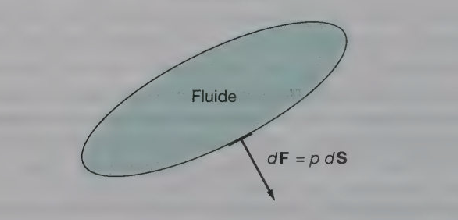
\includegraphics[width=0.6\textwidth]{./assets/Pression.png}
  \caption{Pression}
\end{figure}

\subsection{Travail de pression} % (fold)
\label{sub:Travail de pression}

(On considére $p_0$ uniforme) 
\begin{equation}
  \delta W _{p} = - P_0 \mathrm{d}V
\end{equation}
% subsection Travail de pression (end)
\newpage
\section{Champ de pression d'équilibre d'un fluide} % (fold)
\label{sec:Champ de pression d'équilibre d'un fluide}




\subsection{Opérateur gradient} % (fold)
\label{sub:Opérateur gradient}

\begin{equation}
  \mathrm{d} f = \overrightarrow{\mathrm{grad}} f(M) . \mathrm{d} \overrightarrow{OM}
\end{equation}
% subsection Opérateur gradient (end)
% section Champ de pression d'équilibre d'un fluide (end)

% chapter Pression des fluides (end)

\subsection{Densité volumique de forces} % (fold)

\begin{equation}
  \mathrm{d} \overrightarrow{F} = - \overrightarrow{\mathrm{grad}} P(M) .\mathrm{d}V_M
\end{equation}

ou on dit qu'un système élémentaire subissait une \textbf{force volumique} : 
\begin{equation}
  \overrightarrow{f_v} = - \overrightarrow{\mathrm{grad}} P(M)
\end{equation}

\subsubsection{Champ du poids} % (fold)
\label{sec:Champ du poids}

\begin{equation}
  \overrightarrow{\mathrm{grad}} P(M) = \rho(M) . \overrightarrow{g}(M) \implies \frac{\partial P}{\partial z}  = - \rho g
\end{equation}

\subsubsection{Gaz parfait isotherme} % (fold)

\begin{equation}
  P(z) = P(0) \exp \left( - \frac{Mgz}{RT}  \right)
\end{equation}

% subsubsection Gaz parfait isoterme (end)
% subsubsection Champ du poids (end)

\section{Pousée d'Archimède} % (fold)
\label{sec:Pousée d'Archimède}

Propriété d'une force de pression : ne dépend que la surface et de la pression \underline{du fluide}.

Donc, 
\begin{equation}
  \overrightarrow{F_A} + M _{fl} \overrightarrow{g} = \overrightarrow{0}
\end{equation}
% section Pousée d'Archimède (end)

\section{Tension superficielle} % (fold)
\label{sec:Tension superficielle}

\subsection{Force de tension superficielle} % (fold)
\label{sub:Force de tension superficielle}
\begin{equation}
  \mathrm{d} \overrightarrow{F} _{ts} = \gamma \mathrm{d}l \overrightarrow{n_M}
\end{equation}
% subsection Force de tension superficielle (end)

\subsection{Loi de Laplace} % (fold)
\label{sub:Loi de Laplace}

\begin{equation}
  P _{i}= P_e  + \frac{2 \gamma}{R} 
\end{equation}
% subsection Loi de Laplace (end)
% section Tension superficielle (end)

\newpage
\section{Modèle microscopique de la pression} % (fold)
\label{sec:Modèle microscopique de la pression}

\subsection{Hypothèse} % (fold)
\label{sub:Hypothèse}

Un \textbf{gaz parfait} (GP) est un gaz sans :
\begin{itemize}

    \item volume des molécules
    \item interaction mutuelles entre les molécules

\end{itemize}

\subsection{Températeur cinétique} % (fold)
\label{sub:Températeur cinétique}

On admet que 
\begin{equation}
  \langle E_c \rangle = \frac{3}{2} k_BT \text{ avec } \langle E_c \rangle = \langle \frac{1}{2} m v ^{2} \rangle = \frac{1}{2}  m v ^{*2}
\end{equation}
% subsection Températeur cinétique (end)
% subsection Hypothèse (end)

Donc, 
\begin{equation}
  \boxed{T = \frac{m v ^{*2}}{3 k_B} = \frac{M v ^{*2}}{3 R}, \; v ^{*} = \sqrt{\frac{3RT}{M} } }
\end{equation}
% section Modèle microscopique de la pression (end)

En notant la \textbf{constante des gaz parfaits} : 
\begin{equation}
  \boxed{R = N_A k_B = 8,314 \mathrm{J}. \mathrm{K} ^{-1}. \mathrm{mol} ^{-1}}
\end{equation}
% chapter Densité volumique de forces (end)

\subsection{Pression cinétique} % (fold)

Notons $n ^{*}$ le nombre de particules par unité de volumne (uniforme). On modélise le gaz parfait comme :
\begin{itemize}

    \item Nombre de atomes frappent la surface $\Sigma$ entre $t$ et $t + \mathrm{d} t$ : 
      \begin{equation}
        \mathrm{d} N = n ^{*} \mathrm{d}V = n ^{*} v \mathrm{d} t \mathrm{d} S
      \end{equation}

    \item Changement de la \underline{quantité de mouvement} : 
      \begin{equation}
        \mathrm{d} \Pi = \frac{n ^{*} v \mathrm{d}t \mathrm{d}S}{6}  \times (-2m v) \overrightarrow{e_x}
      \end{equation}

    \item Principe fondamentale de la dymanique : 
      \begin{equation}
        \mathrm{d} \overrightarrow{F} _{\Sigma \to \text{paroi}}= {\color{red} -} P \mathrm{d} S \overrightarrow{e_x} = \frac{\mathrm{d} \Pi}{\mathrm{d} t} = - \frac{1}{3}  n ^{*} mv ^{2} \mathrm{d}S \overrightarrow{e_x} = \frac{\mathrm{d} \Pi}{\mathrm{d} t} = - \frac{1}{3}  n ^{*} mv ^{*2} \mathrm{d}S \overrightarrow{e_x}
      \end{equation}

    \item \textbf{Pression cinétique} : 
      \begin{equation}
        P = \frac{1}{3}  n ^{*} m v ^{*2} = \frac{2n ^{*}}{3}  \langle E _{c} \rangle
      \end{equation}

    \item Conclusion : 
      \begin{equation}
        P = n ^{*}k_B \times T \iff PV = nk_BN_AT = nRT
      \end{equation}

\end{itemize}

Finalement, on a 
\begin{equation}
  PV = nRT
\end{equation}

Plus généralement, dans un corps pur sous une phase, il existe une relation $f(p, V, T) = 0$ appelée \textbf{fonction d'état}.
% subsection Presion cinétique (end)
        
\chapter{Premier Principe de la thermodynamique} % (fold)
\label{chap:Premier Principe de la thermodynamique}

\section{Énergie interne, Enthalpie} % (fold)
\label{sec:Énergie interne}

\subsection{Définitions} % (fold)


\begin{Definition}[colbacktitle=red!75!black]{Énergie interne}{}
L'\textbf{énergie interne} $U$ est la somme des 
\begin{itemize}

    \item énergie cinétiques \underline{microscopiques} des particules de fluide

    \item énergie potentielle des \underline{forces d'interactions microscopiques}. 
\end{itemize}

\begin{equation}
  U = \sum_{i}{E _{c,i}} + \sum_{i}{E _{p, i}}
\end{equation}
\end{Definition}

\begin{Definition}[colbacktitle=red!75!black]{Enthalpie}{}
l'\textbf{enthalpie} de $\Sigma$ (d'énergie $u$, de volume $v$ et de pression $p$) est la grandeur d'état : 
\begin{equation}
  H = U + PV
\end{equation}
\end{Definition}




% subsection Définition (end)


\subsection{Capacités thermiques} % (fold)
\label{sub:Capacités thermiques}

\begin{Theorem}{}{}
Les deux paramètres $V$ et $T$ détermine complètement l'énergie interne : 
\begin{equation}
  U = U(V,T)
\end{equation}

Les deux paramètres $P$ et $T$ détermine complètement l'enthalpie : 
\begin{equation}
  H = H(P,T)
\end{equation}
\end{Theorem}

\begin{Definition}[colbacktitle=red!75!black]{Capacité thermique à volume constant}{}
On définit $C_V$ : grandeur extensive
\begin{equation}
  C_V = \left( \frac{\partial U}{\partial T}  \right)_V
\end{equation}
\end{Definition}

Donc, pour deux états : 
\begin{equation}
  (V,T_1) \to (V, T_2) : \quad U_2 - U_1 = \int_{T_1}^{T_2} C_V(V,T) \mathrm{d}T
\end{equation}

\begin{Definition}[colbacktitle=red!75!black]{Capacité thermique à pression constante}{}
On définit $C_P$ : grandeur extensive 
\begin{equation}
  C_P  = \left( \frac{\partial H}{\partial T}  \right)_P
\end{equation}
\end{Definition}


\subsection{Gaz parfait} % (fold)
\label{sub:Gaz parfait}


Cas d'un gaz parfait monochromatique :
\begin{equation}
  U = N \langle E _{c} \rangle = \frac{3}{2} N k_BT = \frac{3}{2} n RT, \quad H = U + PV = \frac{3}{2} nRT + nRT = \frac{5}{2} nRT
\end{equation}
% subsection Cas d'un gaz parfait monochromatique (end)
\begin{Theorem}{Première loi de Joule}{}
L'\textbf{énergie interne molaire} d'un gaz parfait ne dépend que de la \underline{témperature} de celui-ci : 
\begin{equation}
  U_M = U_m(T)
\end{equation} 
\end{Theorem}

Dans le cas d'un gaz parfait monoatomique : 
\begin{equation}
  U = \frac{3}{2} nRT + U_0 \implies C_V = \frac{3}{2} nR
\end{equation}

\begin{Theorem}{Deuxième loi de Joule}{}
Pour un gaz parfait, l'\textbf{enthalpie molaire} ne dépend que de la température : 
\begin{equation}
  H = U(T) + nRT \implies H_m = H_m(T)
\end{equation}
\end{Theorem}

\begin{Theorem}{Relation de Mayer}{}
\begin{equation}
  C _{pm}= \frac{\mathrm{d} H_m}{\mathrm{d}T}  =  \frac{\mathrm{d}U_m}{\mathrm{d}T}  + R \implies C _{pm} - C _{Vm} = R
\end{equation}
\end{Theorem}

Avec le coefficient $\gamma =  C _{pm} / C _{Vm}$ : 
\begin{equation}
  C _{Vm} = \frac{R}{\gamma - 1} , \quad C _{pm} = \frac{\gamma R}{\gamma -1} 
\end{equation}







\subsection{Phase condensée idéale} % (fold)
\label{sub:Phase condensée idéale}

Au cas de la plupart des solides et des liquides, le volume est très peu sensible aux conditions extérieures : Le seul paramètre intensif qui reste significatif est la température : 
\begin{equation}
  U = U(T),\quad C_V = C_V(T)
\end{equation}
% subsection Phase condensée idéale (end)

De plus, dans une transformation : 
\begin{equation}
[H] _{i} ^{f} = [U] _{i} ^{f} + [PV] _{i} ^{f}
\end{equation}

Le deuxième terme associé au produit $PV$ est négligable. 

Donc, nous aurons, avec une notation $C$ :  
\begin{equation}
  C_P = C_V = C
\end{equation}

\underline{Il n'est pas nécessaire de préciser la capacité thermique}, ils sont confondues.
% subsection Gaz parfait (end)


% subsection Capacités thermiques (end)
% section Énergie interne (end)
\section{Premier Principe de la thermodynamique} % (fold)
\label{sec:Premier Principe de la thermodynamique}

\subsection{Transformation quasi-statique} % (fold)
\label{sub:Transformation quasi-statique}

On peut contrôler l'évolution du système de façon à ce qu'il reste homogène à chaque instant. Les état \underline{intérmédiaires} ont des paramètres d'état \underline{bien définis} et on peut le représenter dans un diagramme $PV$.

Sinon, les seuls états simples connus sont les état \underline{initial} et \underline{final}.
% subsection Transformation quasi-statique (end)

\subsection{Transformation iso-} % (fold)
\label{sub:Transformation iso-}

\begin{itemize}

    \item Transformation \textbf{isotherme} : quasi-statique + $T$ du système reste constante
    \item Transformation \textbf{isobare} : quasi-statique + $P$ du système reste constante
    \item Transformation \textbf{isochore} : transformation à volume constant

\end{itemize}
% subsection Transformation iso- (end)


\subsection{Travail algébrique reçu} % (fold)
\label{sub:Travail algébrique reçu}

Le \textbf{travail} élémentaire reçue : 
\begin{equation}
  \delta W = - p _{ext} \mathrm{d} V
\end{equation}

Au cours de la transformation : 
\begin{equation}
  W _{ext}= \int_{V_i}^{V_f} - p\mathrm{d}V
\end{equation}

\begin{figure}[H] %h:当前位置, t:顶部, b:底部, p:浮动页
  \centering
  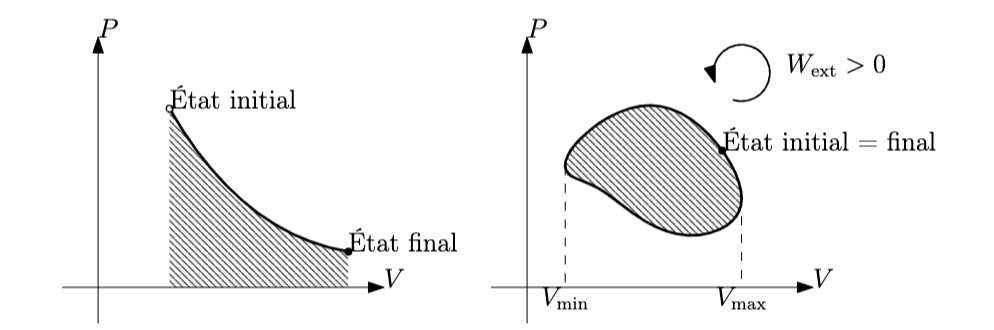
\includegraphics[width=0.8\textwidth]{./assets/Travail des forces de pression.png}
  \caption{Travail des forces de pression}
  \label{fig:Travail des forces de pression}
\end{figure}


Explication : Si $\delta W >0$, le système reçoit du travail, i.e. $\mathrm{d}V < 0$ car le système subit une compression. Sinon, le système subit une détente.
% subsection Travail algébrique reçu (end)

\subsection{Transfert thermique : Chaleur reçu} % (fold)
\label{sub:Transfert thermique : Chaleur reçu}

Le travail que l’extérieur exerce sur le système ne se limite pas au travail macroscopique décrit précédemment. Il existe également les interactions entre les très nombreux atomes du milieu extérieur et ceux de notre système ($\Sigma$), au niveau microscopique. Ces interactions, et leur travail, sont très complexes et il est impossible de les calculer ou de les mesurer directement à partir de données macroscopiques. Pourtant, elles contribuent aussi à la variation de l’énergie mécanique totale du système. 

Nous appelerons cet apport : le \textbf{transfert thermique} ou la \textbf{chaleur}.
% subsection Transfert thermique : Chaleur reçu (end)

\subsection{Énoncé} % (fold)
\label{sub:Énoncé}

\begin{Theorem}{Premier principe de la thermodynamique}{}
Les variations d'énergie mécanique d'un système fermé sont dues seulement au :
\begin{itemize}

    \item travail reçu 
    \item tranfert thermique reçu

\end{itemize}

\begin{equation}
  \Delta E _{tot} = [E _{c,\text{macro} } + U] _i ^{f} = W _{ext} + Q _{ext}
\end{equation}
\end{Theorem}

\subsection{Applications} % (fold)
\label{sub:Applications}

\begin{itemize}

    \item Transformation adiabatique : $Q = 0$ donc $\Delta U = W$ 
    \item Transformation isochore $\mathrm{d} U = 0$ donc $W = 0$, par conséquent $\Delta U = Q$
    \item Transformation monobare : utilisons l'\textbf{enthalpie}, $\Delta H = \Delta (U+PV) = Q$

\end{itemize}
% subsection Applications (end)


% subsection Énoncé (end)

% section Premier Principe de la thermodynamique (end)
% chapter Premier Principe de la thermodynamique (end)

\newpage
\section{Transformations Typiques} % (fold)
\label{sec:Transformations Typiques}

\subsection{Calorimétrie} % (fold)
\label{sub:Calorimétrie}

La méthode : 
\begin{itemize}

    \item Système étudié subit une transformation monobare : $Q = \Delta H$ 
    \item Système thermiquement isolé : $Q = 0$ 
    \item Équation : 
      \begin{equation}
        \sum_{i}^{} \Delta H_i = \Delta H _{\text{eau}} + \Delta H _{\text{calori}} + \dots = 0
      \end{equation}

\end{itemize}
% subsection Calorimétrie (end)
\subsection{Détente de Joule-Gay-Lussac} % (fold)
\begin{figure}[H] %h:当前位置, t:顶部, b:底部, p:浮动页
  \centering
  \includegraphics[width=0.8\textwidth]{./assets/Détente de Joule-Gay-Lussac.png}
  \caption{Détente de Joule-Gay-Lussac}
\end{figure}

On procède par :
\begin{itemize}
    \item Système au repos : $W = 0$, calorifugé : $Q = 0$
    \item Premier principe : $[U] _i ^{f}= 0$ 
    \item Gaz parfait : $U(T_i) = U(T_f)$ donc $T_i = T_f$ 


\end{itemize}

\subsection{Détente de Joule-Thomson} % (fold)
\label{sub:Détente de Joule-Thomson}

\begin{figure}[H] %h:当前位置, t:顶部, b:底部, p:浮动页
  \centering
  \includegraphics[width=0.8\textwidth]{./assets/Détente de Joule-Thomson.png}
  \caption{Détente de Joule-Thomson}
  \label{fig:Détente de Joule-Thomson}
\end{figure}

La détente de Joule-Thomson : 
\begin{itemize}

    \item fluide s'écoule très lentement 
    \item pression différente : $P_e > P_s$
    \item Régime permenant
    \item Parois calorifugée

\end{itemize}

On analyse : 
\begin{itemize}

    \item Premier principe :
      \begin{equation}
        [E _{c, \text{macro}} + U] _t ^{t + \mathrm{d}t} = W _{ext}
      \end{equation}

    \item Travail : 
      \begin{equation}
        W _{ext} = P_e V _{A A'} - P_s V _{B B'}
      \end{equation}

    \item En RP, énergie interne : 
      \begin{equation}
        [U]_t ^{t + \mathrm{d}t} = U _{BB'} - U _{A A'}
      \end{equation}

    \item De même pour l'énergie cinétique (macroscopique)
    \item La masse reste inchangée, car le système est fermé : 
      \begin{equation}
        M _{A A'} = M _{B B'}
      \end{equation}
    \item Le bilan d'énergie : 
      \begin{equation}
        \frac{E _{c, \text{macro}, A A'}}{M _{A A'}}  + \frac{U + P_e  V _{A A'}}{M _{A A'}}  = 
        \frac{E _{c, \text{macro}, BB'}}{M _{BB'}}  + \frac{U + P_s V _{BB'}}{M _{BB'}}   
      \end{equation}

    \item Donc, 
      \begin{equation}
        \frac{v_e ^{2}}{2}  + h_e = \frac{v_s ^{2}}{2}  + h_s
      \end{equation}

    \item Variation d'énergie cinétique massique est négligeable, donc nous aurons 
      \begin{equation}
        h_e = h_s
      \end{equation}
      conservation de l'enthalpie massique. De même, elle ne fait pas varier sa température.
\end{itemize}





% subsection Détente de Joule-Thomson (end)

\subsection{Transformation adiabatique quasi-statique : Loi de Laplace} % (fold)
\label{sub:Transformation adiabatique quasi-statique}

\begin{figure}[H] %h:当前位置, t:顶部, b:底部, p:浮动页
  \centering
  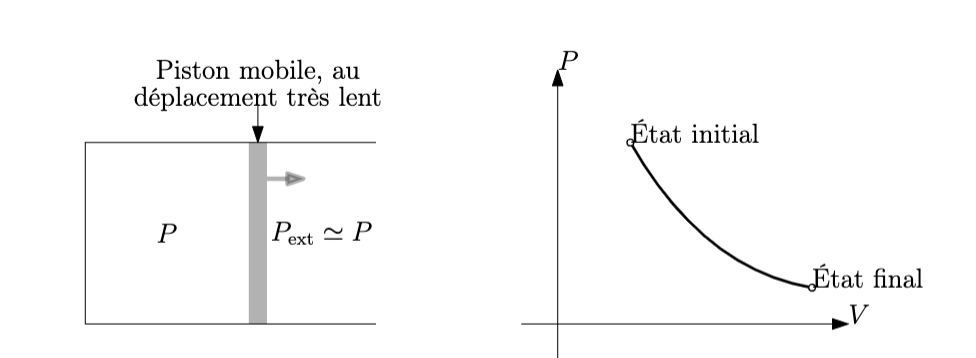
\includegraphics[width=0.8\textwidth]{./assets/Transformation adiabatique quasi-statique d'un gaz parfait.png}
  \caption{Transformation adiabatique quasi-statique d'un gaz parfait}
  \label{fig:Transformation adiabatique quasi-statique d'un gaz parfait}
\end{figure}

On procède comme :
\begin{itemize}

    \item Premier Principe : 
      \begin{equation}
        [U] _t ^{t + \mathrm{d}t} = - p \mathrm{d}V
      \end{equation}

    \item Propriété d'un gaz parfait : 
      \begin{equation}
        \mathrm{d} U = C_V \mathrm{d}T
      \end{equation}

    \item Par ailleurs 
      \begin{equation}
        T = \frac{PV}{nR}  \implies \mathrm{d}T = \frac{1}{nR} (p \mathrm{d}V + V \mathrm{d}p)
      \end{equation}

    \item Enfin, 
      \begin{equation}
        C_v \mathrm{d}T = - p \mathrm{d}V \implies \boxed{\frac{\mathrm{d}p}{p}  + \gamma \frac{\mathrm{d}V}{V} = 0}
      \end{equation}

    \item Ensuite, 
      \begin{equation}
       \mathrm{d} \ln (PV ^{\gamma}) = 0 \implies PV ^{\gamma} = \text{cte}
      \end{equation}


    
\end{itemize}

    On obtient :
    \begin{Theorem}{
        Loi de Laplace : transformation adiabatique quasi-statique
      }{}
    \begin{equation}
      PV ^\gamma = \text{cte}, \quad TV ^{\gamma-1} = \text{cte}, \quad P ^{1-\gamma} T ^\gamma = \text{cte}
    \end{equation}
    \end{Theorem}

% subsection Transformation adiabatique quasi-statique (end)

    \subsubsection{Conséquence du loi de Laplace} % (fold)
    \label{sec:Conséquence du loi de Laplace}
   \begin{Definition}[colbacktitle=red!75!black]{Coefficient de compressibilité isotherme}{}
   \begin{equation}
     \chi_T = - \frac{1}{V}  \left( \frac{\partial V}{\partial P}  \right)_T
   \end{equation}
   Pour une petite variation de $\Delta P$, on observe une changement : 
   \begin{equation}
     \Delta V = - \chi_T V_0 \Delta P
   \end{equation}
   \end{Definition}

   \begin{Definition}[colbacktitle=red!75!black]{
       Coefficient de compressibilité isentropique
     }{}
   \begin{equation}
     \chi_S = - \frac{1}{V}  \left( \frac{\partial V}{\partial P}  \right)_S
   \end{equation}
   \end{Definition}

   
   Pour un gaz parfait : 
   \begin{itemize}

       \item isotherme : 
         \begin{equation}
           PV = nRT= \text{cte} \implies V = \frac{P_0 V_0}{P}         
         \end{equation}

       \item isentropique : 
         \begin{equation}
           PV ^{\gamma} = \text{cte} \implies V = \frac{P_0 ^{1/ \gamma}V_0}{P ^{1/\gamma}} 
         \end{equation}

        \item On a toujours 
          \begin{equation}
            \chi_T = \gamma \chi_S
          \end{equation}

   \end{itemize}

    
    % subsubsection Conséquence du loi de Laplace (end)


% subsection D'etente de Joule-Gay-Lussac (end)
% section Transformations Typiques (end)

\chapter{Deuxième principe de la thermodynamique} % (fold)
\label{chap:Deuxième principe. Bilans d'entropie}

\textbf{Introduction} : Le premier principe (conservation de l’énergie) pose des limites sur les transformations thermodynamiques acceptables : pour un système isolé, une transformation de l’état (a) à l’état (b) n’est possible que si U(a) = U(b) ou, dit autrement, si $\Delta U = 0$. D’après le premier principe, si la transformation de (a) vers (b) est possible, alors celle de (b) vers (a) l’est également.

Cependant, l’expérience montre qu’il n’existe pour chaque système (et chaque choix de U, V, N, etc.) qu’un seul état d’équilibre bien déterminé, et que tout système isolé évolue spontanément et de manière irréversible vers cet état d’équilibre. Le premier principe de la thermodynamique ne suffit pas pour expliquer cette observation, et l’on a besoin d’un second principe pour déterminer l’état d’équilibre. 


\section{Entropie} % (fold)
\subsection{Macro-état et macro-état d'un système} % (fold)
\label{sub:Macro-état et macro-état d'un système}

\subsection{Définition statistique de l'entropie} % (fold)
\label{sub:Définition statistique de l'entropie}

\begin{Theorem}{Formule de Boltzmann}{}
\begin{equation}
  S = k_B \ln \Omega
\end{equation}

où $\Omega$ le nombre d'états microscopiques différents décrivant l'état macroscopique considéré.
\end{Theorem}



% subsection Définition statistique de l'entropie (end)

% subsection Macro-état et macro-état d'un système (end)

% section Entropie (end)
\label{sec:Fonction d'état entropie}


\subsection{Grandeurs d'état entropie} % (fold)
\label{sub:Grandeurs d'état entropie}


\subsubsection{Fonction d'état fondamentale} % (fold)
\label{sec:Fonction d'état fondamentale}

L'entropie est une grandeur d'état qui peut être exprimée en fonction de deux autres grandeurs. 
\begin{equation}
  (U, V) \to S(U,V) \text{ vérifiant } S = S(U,V)
\end{equation}

% subsubsection Fonction d'état fondamentale (end)

\subsubsection{Identité fondamentale} % (fold)
\label{sec:Identité fondamentale}

\begin{equation}
  \left( \frac{\partial S}{\partial U}  \right)_V = \frac{1}{T} , \quad 
  \left( \frac{\partial S}{\partial V}  \right)_U = \frac{P}{T} 
\end{equation}

Au cours d'une petite variation de $\mathrm{d}U$ et $\mathrm{d}V$, on aura 
\begin{equation}
  \mathrm{d}S = \frac{1}{T}  \mathrm{d}U + \frac{P}{T}  \mathrm{d}V = \frac{1}{T}  \mathrm{d}H - \frac{V}{T}  \mathrm{d}P
\end{equation}

\begin{Theorem}{Identités thermodynamique fondamentales}{}
Ils définissent de manière thermodynamique la \underline{pression} et la \underline{température} : 
\begin{equation}
  \boxed{\mathrm{d}U = T \mathrm{d}S - p \mathrm{d} V \implies \mathrm{d}H = T \mathrm{d} S + V \mathrm{d}p}
\end{equation}

Enfin, 
\begin{equation}
  T = \left( \frac{\partial U}{\partial S}  \right)_V, \quad p = -\left(  \frac{\partial U}{\partial V}  \right)_S
\end{equation}
\end{Theorem}

\begin{myproof}{}{}
\begin{equation}
  \mathrm{d} f(x,y) =  \frac{\partial f}{\partial x}  \mathrm{d}x + \frac{\partial f}{\partial y}  \mathrm{d}y
\end{equation}
\end{myproof}





% subsubsection Identité fondamentale (end)

% subsection Grandeurs d'état entropie (end)

\subsubsection{Paramètres pratiques} % (fold)
\label{sec:Paramètres pratiques}

\begin{equation}
  \left( \frac{\partial S}{\partial T}  \right)_V = \frac{C_V}{T} , \quad 
  \left( \frac{\partial S}{\partial T}  \right)_P = \frac{
    C_P
  }{T} 
\end{equation}

\begin{myproof}{}{}

1. 
  \begin{gather}
    S(T, V) = S(U(T, V), V)
  \end{gather}
  2.
\begin{gather}
  S= S(U, V) = S(U(P, T), V(P, T)) \\ 
  \left( \frac{\partial S}{\partial T}  \right)_P = \left( \frac{\partial S}{\partial U}  \right)_V \left( \frac{\partial U}{\partial T}  \right)_P + \left( \frac{\partial S}{\partial V}  \right)_U + \left( \frac{\partial V}{\partial T}  \right)_P = \frac{1}{T} \left( \frac{\partial (U + PV)}{\partial T}  \right)_P
\end{gather}
\end{myproof}


% subsubsection Paramètres pratiques (end)


% subsection  (end)
\subsection{Entropie d'un gaz parfait} % (fold)
\label{sub:Entropie d'un gaz parfait}

\subsubsection{Couplage $(V,T)$} % (fold)

% subsubsection Couplage $(V,T)$ (end)

Pour un gaz parfait, $C_V$ ne dépend que $T$. 

\begin{gather}
  S(T, V) = S(T_0, V_0) + nR \ln \left( \frac{V}{V_0}  \right) + \frac{nR}{\gamma - 1}  \ln \left( \frac{T}{T_0}  \right)
\end{gather}

\begin{myproof}{}{}
  \begin{align}
    \mathrm{d}S &= \frac{1}{T} \mathrm{d} T + \frac{P}{T} \mathrm{d} V \\  
                &= \frac{C_V}{T} \mathrm{d}T + \frac{nR}{V}  \mathrm{d} V
  \end{align}
  Donc, 
  \begin{equation}
    \Delta S = \int_{T}^{} C_V \ln \left( \frac{T}{T_0}  \right)+ \int_{V}^{} nR \ln\left( \frac{V}{V_0}  \right)
  \end{equation}
\end{myproof}

\subsubsection{Couplage $(P,V)$} % (fold)
\label{sec:Couplage $(P,V)$}

Pour un gaz parfait, 
\begin{equation}
  S(P,V) = S(P_0, V_0) + \frac{nR}{\gamma-1}  \left[ \ln \left( \frac{P_2}{P_1}  \right) + \gamma \ln \left( \frac{V_2}{V_1}  \right) \right]
\end{equation}

\begin{myproof}{}{}
\begin{note}{}{}
Différencier logarithmiquement l'équation d'état $PV = nRT$ : 
\begin{equation}
  \frac{\mathrm{d}p}{p}  +  \frac{\mathrm{d}V}{V} = \frac{\mathrm{d}T}{T} 
\end{equation}
\end{note}

Donc, 
\begin{align}
  \mathrm{d} S &= \frac{nR}{\gamma-1} \frac{\mathrm{d}T}{T}  + nR \frac{\mathrm{d}V}{V}  \\ 
               &= \left( \frac{nR}{\gamma-1}  \right) \left( \frac{\mathrm{d}p}{p}  + \left( \frac{\mathrm{d}V}{V}  \right) \right) + nR \frac{\mathrm{d}V}{V}  \\ 
               &= \frac{nR}{\gamma-1}  \left( \frac{\mathrm{d}p}{p}  + \gamma \frac{\mathrm{d}V}{V}  \right)
\end{align}


\end{myproof}


% subsubsection Couplage $(P,V)$ (end)


% subsection Entropie d'un gaz parfait (end)

\subsection{Entropie d'une phase condensée idéale} % (fold)
\label{sub:Entropie d'une phase condensée idéale}
Comme $V$ est presque inchangé,  le seule paramètre est la température : 
\begin{equation}
  S(T) = S(T_0) + \int_{T_0}^{T} \frac{C_V(T')}{T'}  \mathrm{d}T '
\end{equation}

Dans le cas de capacité thermique constante :
\begin{equation}
  S(T) = S(T_0) + C \ln \left( \frac{T}{T_0}  \right)
\end{equation}
% subsection Entropie d'une phase condensée idéale (end)
% section Fonction d'état entropie (end)

\newpage
\section{Deuxième principe de la thermodynamique} % (fold)
\label{sec:Deuxième principe de la thermodynamique}

\subsection{Énoncé} % (fold)
\label{sub:Énoncé}


\textbf{Principe d'évolution} : L'entropie d'un \underline{système isolé} ne peut \underline{qu}'\underline{augmenter} ou \underline{rester constante} au cours du temps.
% subsection Énoncé (end)

\subsection{Équilibre thermodynamique d'un système isolé} % (fold)
\label{sub:Équilibre thermodynamique d'un système isolé}

Un état d'équilibre d'un système isolé est un état dans lequel l'entropie est \underline{maximale}.
% subsection Équilibre thermodynamique d'un système isolé (end)

\subsubsection{Exemple} % (fold)
\label{sec:Exemple}

[fig]
On doit avoir  
\begin{equation}
  T_1 = T_2
\end{equation}

\begin{myproof}{}{}
\begin{gather}
  S = S(U_1, V_1) + S(U_2, V_2) = S(U_1, V_1) + S(U_0 - U_1, V_2) \\ 
  \frac{\mathrm{d}S}{\mathrm{d}U_1} = \frac{1}{T_1(U_1, V_1)} - \frac{1}{T_2(U_0-U_1, V_2)}  = 0
\end{gather}
\end{myproof}

Si $T_1>T_2$, comme $S$ augmente en même temps, $U_1$ ne peut que diminuer.


% subsubsection Exemple (end)


\subsection{Transformation réversible} % (fold)
\label{sub:Transformation réversible}

\subsubsection{Transformation quasi-statique} % (fold)
\label{sec:Transformation quasi-statique}

% subsubsection Transformation quasi-statique (end)

\subsubsection{Transformation isentropique} % (fold)
\label{sec:Transformation isentropique}

Exemple : Transformation adiabatique quasi-statique d'un gaz parfait. 
\begin{equation}
  \mathrm{d}U = - P \mathrm{d} V \implies \mathrm{d}S = \frac{\mathrm{d}U + P \mathrm{d}V}{T}  = 0 
\end{equation}
% subsubsection Transformation isentropique (end)

\subsubsection{Entropie créée} % (fold)
\label{sec:Entropie créée}

L'\textbf{entropie créée} nous permet de quantifier le caractère réversible ou non : 
\begin{equation}
  S _{cr} = [S] _{i} ^{f}
\end{equation}

D'après le deuxième principe : 
\begin{equation}
  S _{cr} \ge _{rev} 0
\end{equation}
% subsubsection Entropie créée (end)
% subsection Transformation réversible (end)

% section Deuxième principe de la thermodynamique (end)

\section{Bilan entropique} % (fold)
\label{sec:Bilan entropique}

\subsection{Source de chaleur} % (fold)
\label{sub:Source de chaleur}

\begin{equation}
  [S _{th}] _i ^{f} = \frac{Q _{th}}{T_0} 
\end{equation} 
% subsection Source de chaleur (end)

\subsection{Système en contact avec une source de chaleur} % (fold)
\label{sub:Système en contact avec une source de chaleur}

\begin{equation}
  [S] _{i} ^{f} = S _{cr} + S _{ech}
\end{equation}
% subsection Système en contact avec une source de chaleur (end)

\subsection{Contact avec plusieurs thermostat} % (fold)
\label{sub:Contact avec plusieurs thermostat}

\begin{equation}
  S _{ech} = \sum_{i}^{} \frac{Q_i}{T_i} 
\end{equation}
% subsection Contact avec plusieurs thermostat (end)
% section Bilan entropique (end)


% chapter Deuxième principe. Bilans d'entropie (end)

\chapter{Changement de Phase} % (fold)
\label{chap:Changement de Phase}

\section{Diagramme d'équilibre} % (fold)
\label{sec:Diagramme d'équilibre}

\begin{figure}[H] %h:当前位置, t:顶部, b:底部, p:浮动页
  \centering
  \includegraphics[width=\textwidth]{./assets/Diagramme (P,T) dans le cas général puis dans le cas particulier de l'eau.png}
  \caption{Diagramme (P,T) dans le cas général puis dans le cas particulier de l'eau}
  \label{fig:Diagramme (P,T) dans le cas général puis dans le cas particulier de l'eau}
\end{figure}

Mémoire : considérer $PV = nRT \implies \rho =PM/RT$


\section{Enthalpie} % (fold)
\label{sec:Enthalpie}

\subsection{Enthalpie de changement de phase} % (fold)
\label{sub:Enthalpie de changement de phase}

Deux phases 1 et 2 existent à $T$ et une pression $P = P _{eq}(T)$. 

On appelle \textbf{enthalpie molaire de changement de phase} (1 vers 2) : 
\begin{equation}
  \Delta _{12} H_m(T) = H _{m2} (T , P _{eq}(T)) - H _{m1}(T, P _{eq}(T))
\end{equation}

\subsubsection{Transformation monobare} % (fold)
\label{sec:Transformation monobare}
\begin{itemize}

    \item Premier principe : 
      \begin{equation}
        [H] _i ^{f} = Q _{ext}
      \end{equation}

    \item Variation d'enthalpie : 
      \begin{equation}
        [H] _i ^{f} = n \times\Delta _{12} H_m(T)
      \end{equation}

    \item Finalement,
      \begin{equation}
        \Delta _{12}H_m(T) = \frac{
          Q _{ext}
        }{n} 
      \end{equation}

\end{itemize}
% subsubsection Transformation monobare (end)
\subsubsection{Ordre} % (fold)
\label{sec:Ordre}

% subsubsection Ordre (end)
\textbf{ODG} : $\Delta _{\text{vap}}H_m >0$, $\Delta _{\text{fus}}H_m >0$, $\Delta _{sub} H_m >0$.

Si la phase 2 est plus d'esordonn'ee que la phase 1, alors $\Delta _{12}H_m >0$

% subsection Enthalpie de changement de phase (end)
% section Enthalpie (end)
% section Diagramme d'équilibre (end)

\subsection{Enthalpie d' un sysème biphasé} % (fold)
\label{sub:Enthalpie d' un sysème biphasé}

Soit un corps pur comprenant une quantité $n_1 = X_1n$ et $n_2 = X_2n$, l'enthalpie est :
\begin{equation}
  \boxed{H = n_1 \times H _{m1} + n_2 \times H _{m2}}
\end{equation}

ou encore 
\begin{equation}
  X_2 = \frac{H_m - H _{m1}}{\Delta _{12}H_m} 
\end{equation}
% subsection Enthalpie d' un sysème biphasé (end)

\subsection{Transformation générale} % (fold)
\label{sub:Transformation générale}
L'état initial : phase 1, $T_i$, $P= P _{eq}(T_i)$ à phase 2, $T_f$, $X_{2f}$, $P = P _{eq}(T_f)$ = Transformation monobare + Changement de phase à $(T_f, P = P _{eq}(T_f))$
\begin{equation}
  [H]_i ^{f} = n \times (C _{pm1} \times(T_f - T_i) + X _{2f} \times \Delta _{12}H_m(T_f))
\end{equation}

\begin{figure}[H] %h:当前位置, t:顶部, b:底部, p:浮动页
  \centering
  \includegraphics[width=0.8\textwidth]{./assets/Enthalpie - transformation générale.png}
  \caption{Enthalpie - transformation générale}
\end{figure}

Note : État initial : $T_i, X _{1i} = 1$, État intermédiaire : $T_f, X _{1i}=1$


\section{Entropie} % (fold)
\label{sec:Entropie}


\subsection{Entropie molaire de changement de phase} % (fold)
\label{sub:Entropie molaire de changement de phase}
\begin{equation}
  \Delta _{12} S_m(T) = S _{m2}(T, P _{eq}(T) ) - S _{m1} (T, P _{eq}(T))
\end{equation}
% subsection Entropie molaire de changement de phase (end)

\subsection{Relation avec l'enthalpie} % (fold)
\label{sub:Relation avec l'enthalpie}

\begin{equation}
  \Delta _{12}S_m(T) = \frac{
    \Delta _{12}H_m(T)
  }{T} 
\end{equation}
% subsection Relation avec l'enthalpie (end)
% section Entropie (end)

% subsection Transformation générale (end)
% chapter Changement de Phase (end)

\chapter{Machine Thermique} % (fold)
\label{chap:Machine Thermique}

\section{Transformation cyclique} % (fold)
\label{sec:Transformation cyclique}

\subsection{Moteurs et récpteurs} % (fold)
\label{sub:Moteurs et récpteurs}

% subsection Moteurs et récpteurs (end)

\subsection{Répresentation en diagramme} % (fold)
\label{sub:Répresentation en diagramme}

\subsubsection{Diagramme de Clapeyron} % (fold)
\label{sec:Diagramme de Clapeyron}

% subsubsection Diagramme de Clapeyron (end)
% subsection Répresentation en diagramme (end)

\subsection{Bilans sur un cycle} % (fold)
\label{sub:Bilans sur un cycle}

Au cours d'un cycle, toutes les grandeurs d'état reste inchangée.

\begin{itemize}

    \item Bilan d'énergie interne : 
      \begin{equation}
        [U] _i ^{f} = 0 \implies W + Q = 0
      \end{equation}

    \item Bilan d'entropie : 
      \begin{equation}
        [S] _ i ^{f} = 0 \implies S _{cr} + S _{ech} = 0
      \end{equation}
\end{itemize}
% subsection Bilans sur un cycle (end)

\subsection{Machines monotherme : impossible} % (fold)
\label{sub:Machines monotherme : impossible}

\begin{equation}
  Q = T_0 S _{ech} = - T_0 S _{cr} \le _{rev} 0 \implies W \ge _{rev} 0
\end{equation}

\textbf{Conclusion} : Il est impossible de réaliser un moteur avec un cycle monotherme.
% subsection Machines monotherme : impossible (end)

\subsection{Machines multithermes} % (fold)
\label{sub:Machines multithermes}

\subsubsection{Inégalité de Clausius} % (fold)
\label{sec:Inégalité de Clausius}

\begin{equation}
  \sum_{i}^{} \frac{Q_i}{T_i}  \le _{rev} 0
\end{equation}
% subsubsection Inégalité de Clausius (end)
% subsection Machines multithermes (end)
% section Transformation cyclique (end)

\newpage
\section{Machines dithermes} % (fold)
\label{sec:Machines dithermes}

\begin{tcolorbox}
  \textbf{Notations} : Pendant un cycle, le système $\Sigma$ \underline{reçoit} la chaleur $Q_C$ de la part de la source chaude de température $T_C$, de même façon \underline{reçoit} $Q_F$ de celle de $T_F$.
\end{tcolorbox}
\subsection{Diagramme de Raveau} % (fold)
\label{sub:Diagramme de Raveau}

\begin{figure}[H] %h:当前位置, t:顶部, b:底部, p:浮动页
  \centering
  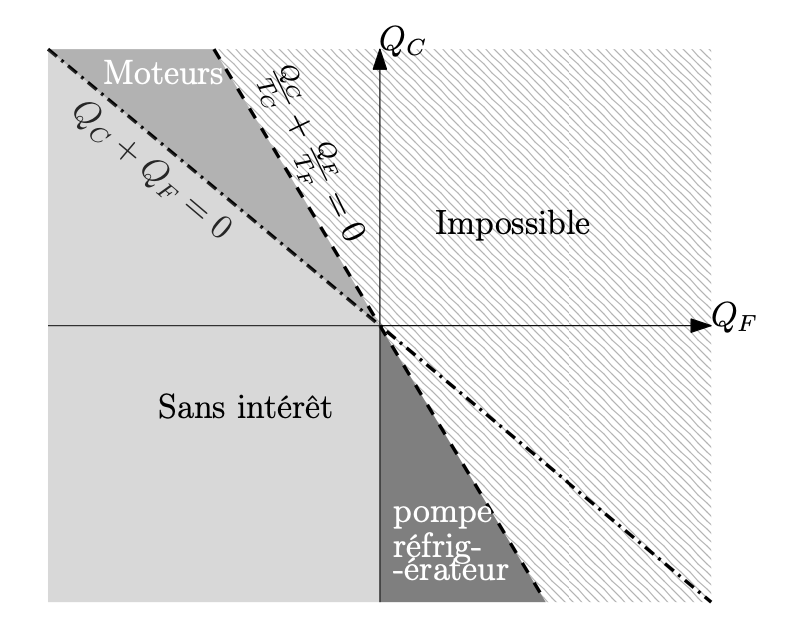
\includegraphics[width=0.6\textwidth]{./assets/Diagramme de Raveau.png}
  \caption{Diagramme de Raveau}
  \label{fig:Diagramme de Raveau}
\end{figure}

Explication : 
\begin{itemize}

    \item Droites :
      \begin{equation}
        \frac{Q_C}{T_C}  + \frac{Q_F}{T_F}  < 0 \implies Q_C < - \frac{T_C}{ T_F}  Q_F \text{ avec } \frac{T_C}{T_F}  > 1
      \end{equation}

    \item La domaine des \underline{moteurs} : 
      \begin{equation}
        Q_C > 0, \; Q_F < 0 ,\; W = - (Q_C + Q_F) < 0
      \end{equation}

    \item La domaine des \underline{récepteurs} : 
      \begin{equation}
        Q_C < 0, \; Q_F > 0, \; W = - (Q_C + Q_F) > 0
      \end{equation} 

\end{itemize}

% subsection Diagramme de Raveau (end)
% section Machines dithermes (end)

\subsection{Efficacité thermodynamique} % (fold)
\label{sub:Efficacité thermodynamique}

\subsubsection{Définition} % (fold)
\label{sec:Définition}

\begin{itemize}

    \item \textbf{Efficacité thermodynamique} : 
      \begin{equation}
        e = \frac{\text{ce que l'on veut}}{\text{ce que l'on paye}} 
      \end{equation} 
    \item \textbf{Rendement} : 
      \begin{equation}
        \eta = \frac{e _{\text{réelle}}}{e _{\text{théorique}}} 
      \end{equation}

\end{itemize}

\subsubsection{Moteur : efficacité de Carnot} % (fold)
\label{sec:Moteur : efficacité de Carnot}

L'efficacité du moteur est limitée par : 
\begin{equation}
  e  = \frac{-W}{Q_C} \le _{rev} e_c = 1 - \frac{T_F}{T_C} 
\end{equation}
% subsubsection Moteur : efficacité de Carnot (end)
% subsubsection Définition (end)
% subsection Efficacité thermodynamique (end)

\subsubsection{Machine frigorifique : efficacité frigorifique de Carnot} % (fold)
\label{sec:Machine frigorifique}

L'efficacité : 
\begin{equation}
  e  = \frac{Q_F}{W}  \le _{rev} e _{fr,c} =  \frac{T_F}{T_C- T_F} 
\end{equation}

\begin{myproof}{}{}
\begin{equation}
  \frac{Q_F}{W}  = \frac{Q_F}{-(Q_F+Q_C)}  = \frac{1}{ - 1 + \frac{Q_C}{Q_F} }  \le _{rev} - \frac{1}{ 1- \frac{T_C}{T_F} } 
\end{equation}
\end{myproof}


\begin{tcolorbox}
    \textbf{Note} : Il faut comprendre que $Q_F$ représente : on \underline{tire le chaleur de la source froide} (à l'intérieur) et de donner de la chaleur à la source chaude. $Q_F$ est considéré chaleur \underline{reçu} donc il est positif.
\end{tcolorbox}
% subsubsection Machine frigorifique (end)


\subsubsection{Pompe à chaleur} % (fold)
\label{sec:Pompe à chaleur}

\begin{equation}
  e = -\frac{Q_C}{W}  \le _{rev} e _{th,c} = \frac{T_C}{T_C - T_F}  
\end{equation}

\begin{tcolorbox}
    \textbf{Note} : On souhaite de \underline{donner de la chaleur à la source chaude} (intérieur, en hiver) en la prélevant à la source froide.
\end{tcolorbox}
% subsubsection Pompe à chaleur (end)

\subsection{Cycle de Carnot} % (fold)
\label{sub:Cycle de Carnot}

\subsubsection{Condition de réversibilité} % (fold)
\label{sec:Condition de réversibilité}

Dans un cycle ditherme \underline{réversible} (isentropique) : 
\begin{itemize}

    \item Quand il échange de chaleur avec un thermostat, la température du système doit rester inchangé. 

    \item La reste du cycle doit être isentropique = adiabatique réversible.

\end{itemize}

Donc, le cycle de Carnot est impossible à réaliser en pratique.

\subsubsection{Représentation pour un gaz parfait} % (fold)
\label{sec:Représentation pour un gaz parfait}

La courbe consiste à deux parties : 
\begin{itemize}

    \item partie isotherme : $PV = nRT_F$ et $PV = nRT_C$ 
    \item partie isentropique : Loi de Laplace donne $PV ^{\gamma} = C _{te}$

\end{itemize}

\begin{figure}[H] %h:当前位置, t:顶部, b:底部, p:浮动页
  \centering
  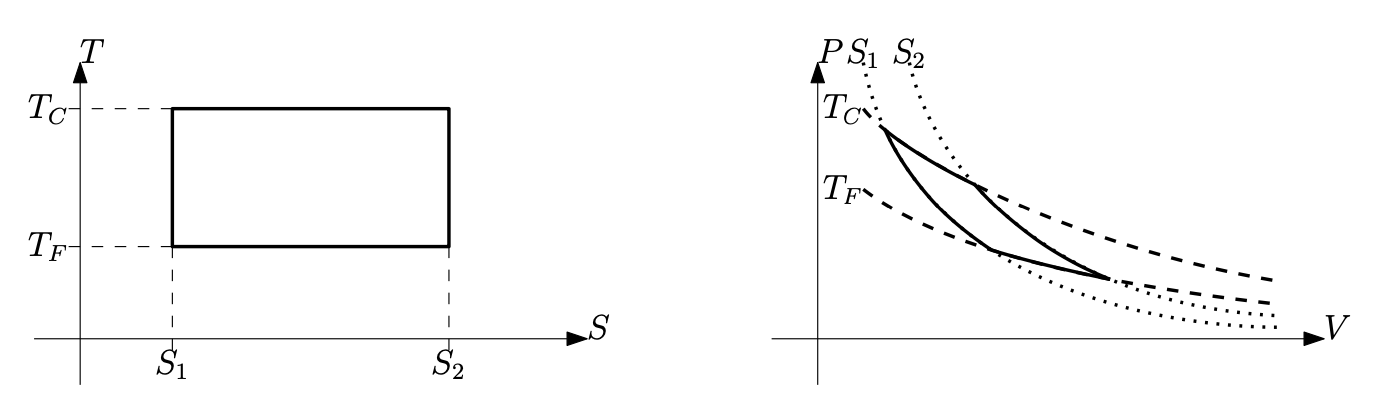
\includegraphics[width=0.8\textwidth]{./assets/Cycle de Carnot (GP).png}
  \caption{Cycle de Carnot (GP)}
  \label{fig:Cycle de Carnot (GP).png}
\end{figure}


% subsubsection Représentation pour un gaz parfait (end)
% subsubsection Condition de réversibilité (end)
% subsection CYcle de Carnot (end)

\subsection{Exemple : Cycle de Beau de Rochas} % (fold)
\label{sub:Exemple : Cycle de Beau de Rochas}

\begin{figure}[H] %h:当前位置, t:顶部, b:底部, p:浮动页
  \centering
  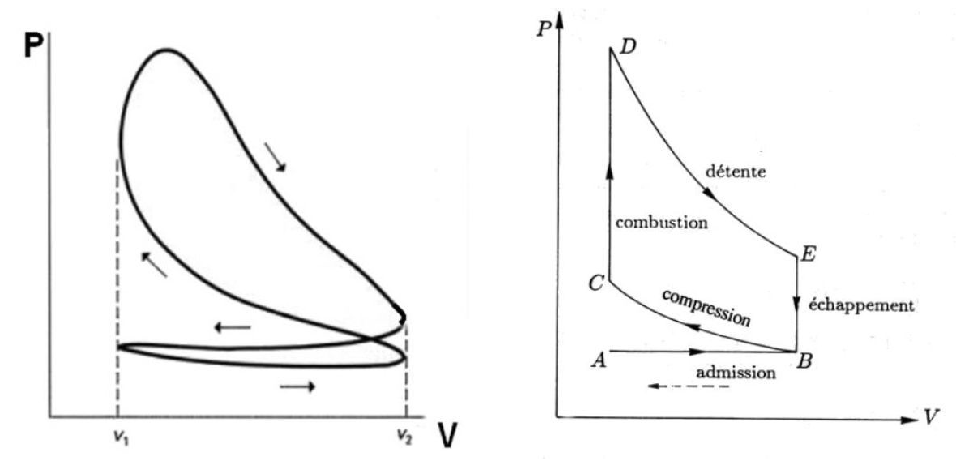
\includegraphics[width=0.8\textwidth]{./assets/Cycle de Beau de Rochas 1.png}
  \caption{Cycle de Beau de Rochas}
\end{figure}

\begin{figure}[H] %h:当前位置, t:顶部, b:底部, p:浮动页
  \centering
  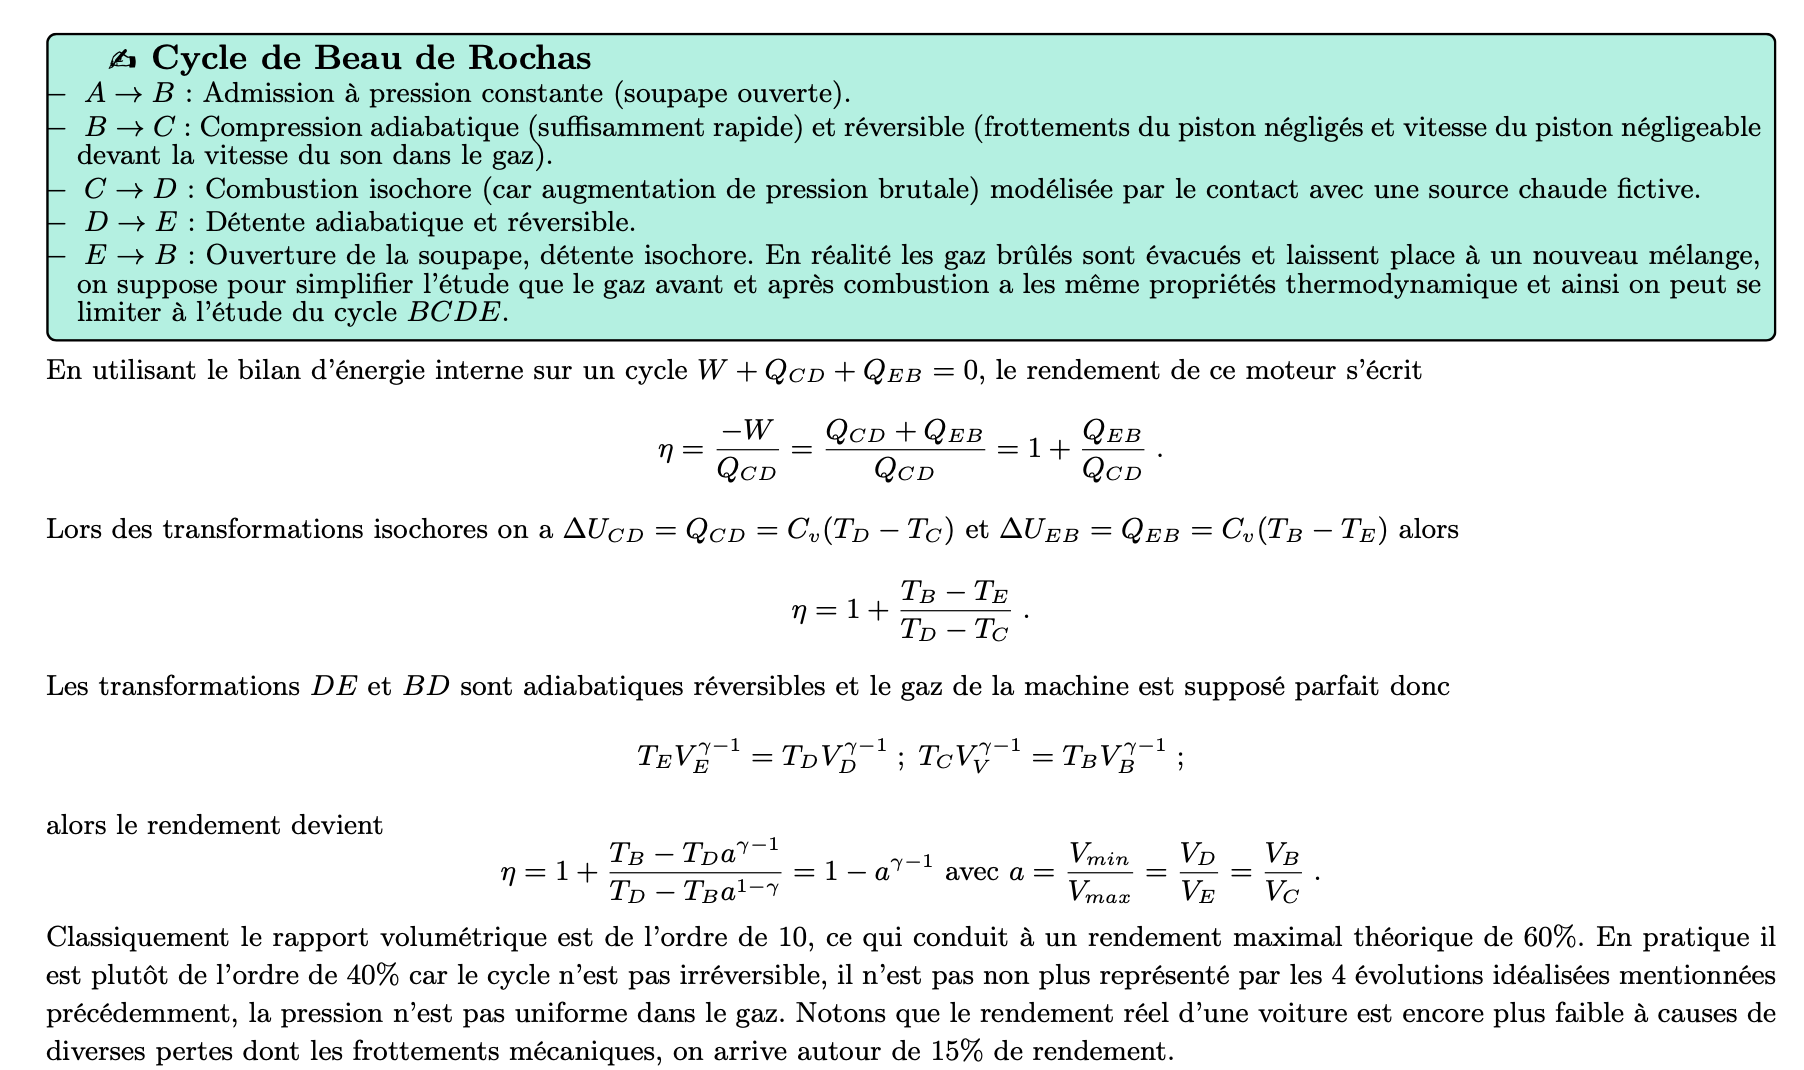
\includegraphics[width=1\textwidth]{./assets/Cycle de Beau de Rochas 2.png}
\end{figure}




% subsection Exemple : Cycle de Beau de Rochas (end)
 (end)
\subsection{Exemple : Machines frigorifiques} % (fold)
\label{sub:Exemple : Machines frigorifiques}

\begin{figure}[H] %h:当前位置, t:顶部, b:底部, p:浮动页
  \centering
  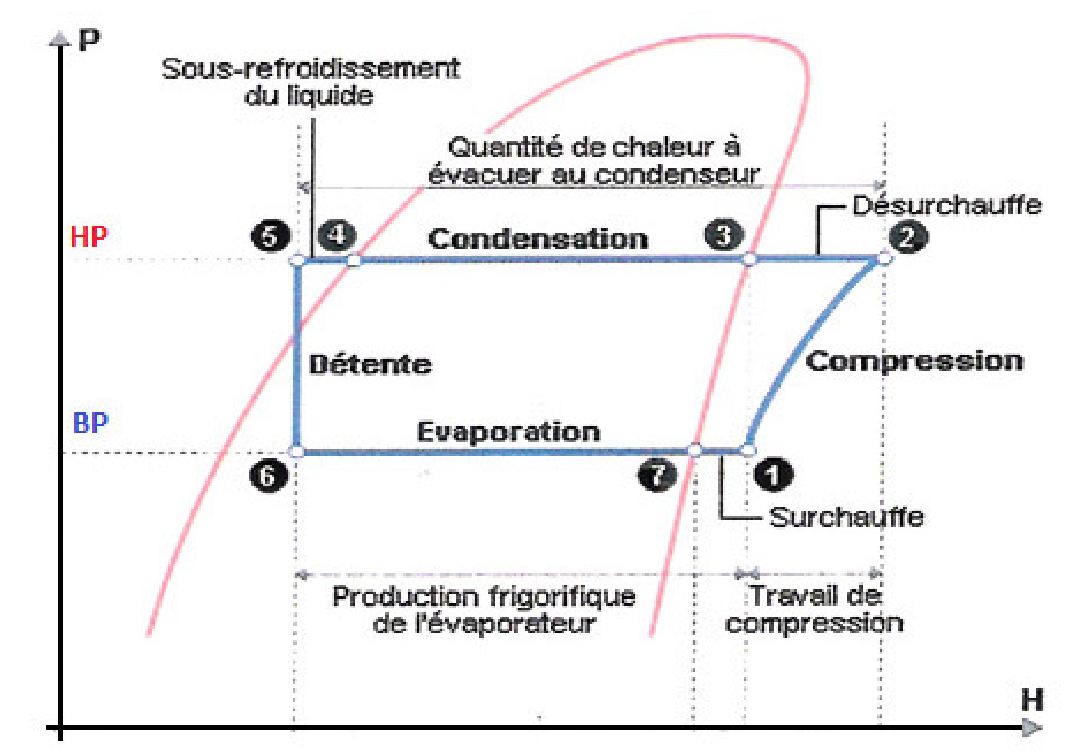
\includegraphics[width=0.8\textwidth]{./assets/Machines frigorifiques 1.png}
  \caption{Machines frigorifiques}
\end{figure}

\begin{figure}[H] %h:当前位置, t:顶部, b:底部, p:浮动页
  \centering
  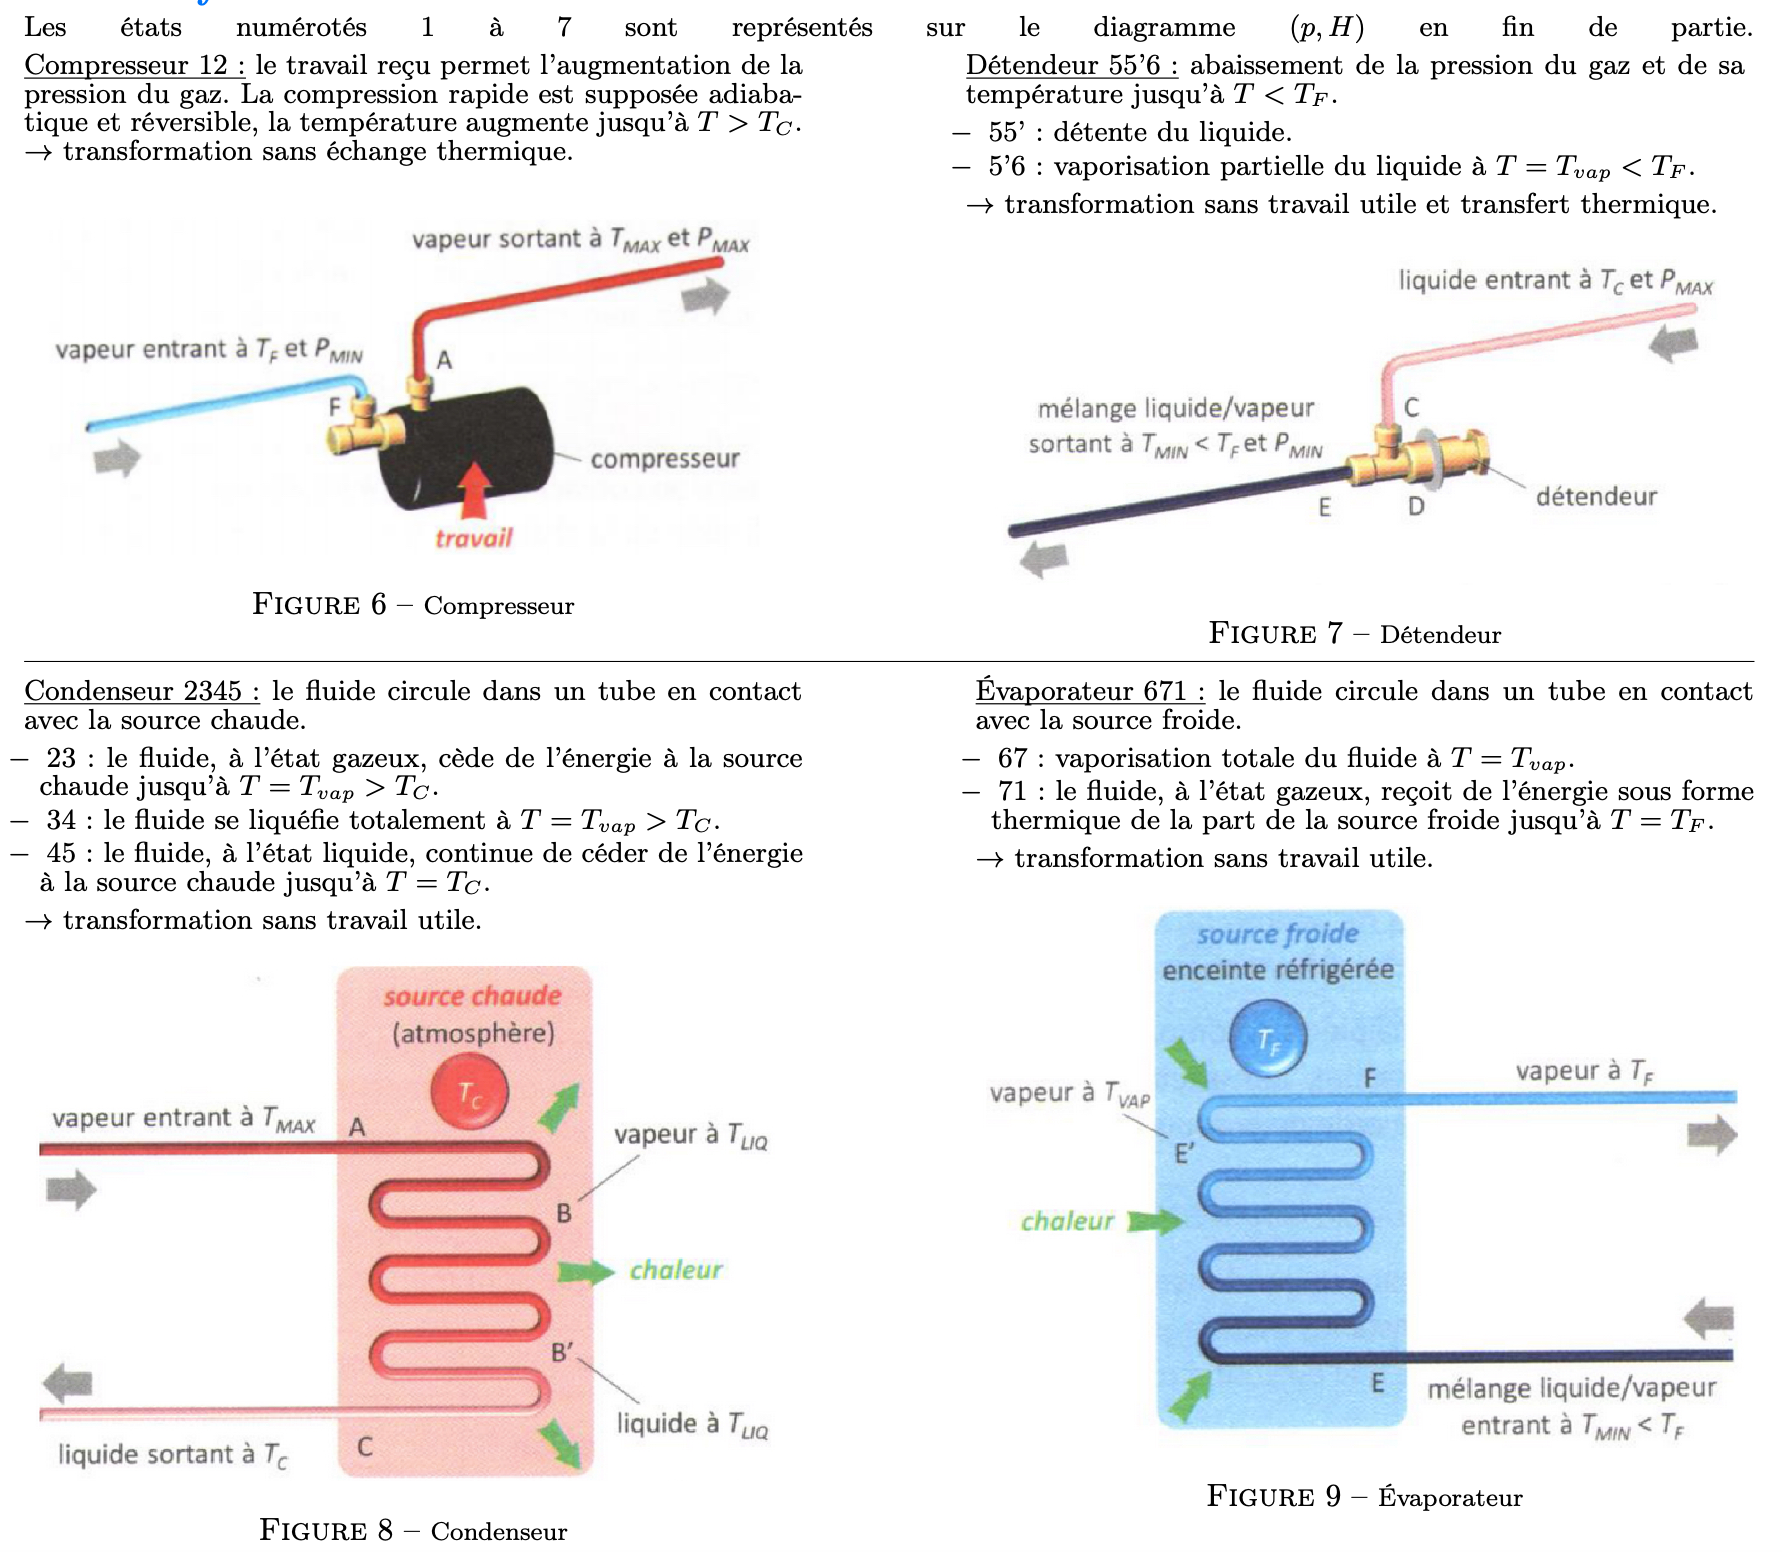
\includegraphics[width=\textwidth]{./assets/Machines frigorifiques 2.png}
\end{figure}



% subsection Exemple : Machines frigorifiques (end)
% section  (end)

\newpage 
\section{Dispositifs avec fluide en écoulement} % (fold)
\label{sec:Dispositifs avec fluide en écoulement}

\subsection{Généralités} % (fold)
\label{sub:Généralités}

\subsubsection{Bilan de masse} % (fold)
\label{sec:Bilan de masse}

% subsubsection Bilan de masse (end)
% subsection Généralités (end)

\begin{figure}[H] %h:当前位置, t:顶部, b:底部, p:浮动页
  \centering
  \includegraphics[width=0.8\textwidth]{./assets/Système d'étude.png}
  \caption{Système d'étude}
  \label{fig:Système d'étude}
\end{figure}




Considérons le système fermé $\Omega$ constitué de la matière qui, à l'instant $t$ se trouve entre $I$ et $O$. Une courte durée $\mathrm{d}t$ plus tard, $\Omega$ se \underline{retrouve} entre $I'$ et $O'$. 

Notons $M ^{*}(t)$ la masse de $\Omega$, à l'instant $t$. 
\begin{itemize}

    \item Système fermé : $M ^{*}( t+ \mathrm{d} t) = M ^{*}(t)$ 
    \item $M ^{*}(t + \mathrm{d} t) = M _{I'O} + M _{OO'}$, $M ^{*}(t) = M _{II'}+ M _{I'O}$

\end{itemize}

En régime permanent, donc $M _{OO' }- M _{II' }= 0$, avec la définition de \textbf{débits massiques} : 
\begin{equation}
  M _{OO'} = D_e \mathrm{d} t, \; M _{II'} = D_s \mathrm{d} t \implies D_e = D_s = D
\end{equation}
% subsection Bilan de masse (end)

\subsubsection{Bilan d'un grandeur extensive quelconque} % (fold)
\label{sec:Bilan d'un grandeur extensive quelconque}

\begin{equation}
  \frac{\mathrm{d}X ^{*}}{ \mathrm{d}t}  = D [x] _{e} ^{s}
\end{equation}
% subsubsection Bilan d'un grandeur extensive quelconque (end)

\subsection{Échange énergétique} % (fold)
\label{sub:Échange énergétique}

Le premier principe : 
\begin{equation}
  \left[ h + \frac{v ^{2}}{2}  \right] _{e} ^{s} = w _{mec} + q
\end{equation}

avec $w _{mec}$ est le travail reçu pour chaque unité de fluide
% subsection Échange énergétique (end)
% section Dispositifs avec fluide en écoulement (end)
% chapter Machine Thermique (end)


\end{document}
